
\documentclass{article} % For LaTeX2e
\usepackage{iclr2027_conference,times}

% Optional math commands from https://github.com/goodfeli/dlbook_notation.
%%%%% NEW MATH DEFINITIONS %%%%%

\usepackage{amsmath,amsfonts,bm}

% Mark sections of captions for referring to divisions of figures
\newcommand{\figleft}{{\em (Left)}}
\newcommand{\figcenter}{{\em (Center)}}
\newcommand{\figright}{{\em (Right)}}
\newcommand{\figtop}{{\em (Top)}}
\newcommand{\figbottom}{{\em (Bottom)}}
\newcommand{\captiona}{{\em (a)}}
\newcommand{\captionb}{{\em (b)}}
\newcommand{\captionc}{{\em (c)}}
\newcommand{\captiond}{{\em (d)}}

% Highlight a newly defined term
\newcommand{\newterm}[1]{{\bf #1}}


% Figure reference, lower-case.
\def\figref#1{figure~\ref{#1}}
% Figure reference, capital. For start of sentence
\def\Figref#1{Figure~\ref{#1}}
\def\twofigref#1#2{figures \ref{#1} and \ref{#2}}
\def\quadfigref#1#2#3#4{figures \ref{#1}, \ref{#2}, \ref{#3} and \ref{#4}}
% Section reference, lower-case.
\def\secref#1{section~\ref{#1}}
% Section reference, capital.
\def\Secref#1{Section~\ref{#1}}
% Reference to two sections.
\def\twosecrefs#1#2{sections \ref{#1} and \ref{#2}}
% Reference to three sections.
\def\secrefs#1#2#3{sections \ref{#1}, \ref{#2} and \ref{#3}}
% Reference to an equation, lower-case.
\def\eqref#1{equation~\ref{#1}}
% Reference to an equation, upper case
\def\Eqref#1{Equation~\ref{#1}}
% A raw reference to an equation---avoid using if possible
\def\plaineqref#1{\ref{#1}}
% Reference to a chapter, lower-case.
\def\chapref#1{chapter~\ref{#1}}
% Reference to an equation, upper case.
\def\Chapref#1{Chapter~\ref{#1}}
% Reference to a range of chapters
\def\rangechapref#1#2{chapters\ref{#1}--\ref{#2}}
% Reference to an algorithm, lower-case.
\def\algref#1{algorithm~\ref{#1}}
% Reference to an algorithm, upper case.
\def\Algref#1{Algorithm~\ref{#1}}
\def\twoalgref#1#2{algorithms \ref{#1} and \ref{#2}}
\def\Twoalgref#1#2{Algorithms \ref{#1} and \ref{#2}}
% Reference to a part, lower case
\def\partref#1{part~\ref{#1}}
% Reference to a part, upper case
\def\Partref#1{Part~\ref{#1}}
\def\twopartref#1#2{parts \ref{#1} and \ref{#2}}

\def\ceil#1{\lceil #1 \rceil}
\def\floor#1{\lfloor #1 \rfloor}
\def\1{\bm{1}}
\newcommand{\train}{\mathcal{D}}
\newcommand{\valid}{\mathcal{D_{\mathrm{valid}}}}
\newcommand{\test}{\mathcal{D_{\mathrm{test}}}}

\def\eps{{\epsilon}}


% Random variables
\def\reta{{\textnormal{$\eta$}}}
\def\ra{{\textnormal{a}}}
\def\rb{{\textnormal{b}}}
\def\rc{{\textnormal{c}}}
\def\rd{{\textnormal{d}}}
\def\re{{\textnormal{e}}}
\def\rf{{\textnormal{f}}}
\def\rg{{\textnormal{g}}}
\def\rh{{\textnormal{h}}}
\def\ri{{\textnormal{i}}}
\def\rj{{\textnormal{j}}}
\def\rk{{\textnormal{k}}}
\def\rl{{\textnormal{l}}}
% rm is already a command, just don't name any random variables m
\def\rn{{\textnormal{n}}}
\def\ro{{\textnormal{o}}}
\def\rp{{\textnormal{p}}}
\def\rq{{\textnormal{q}}}
\def\rr{{\textnormal{r}}}
\def\rs{{\textnormal{s}}}
\def\rt{{\textnormal{t}}}
\def\ru{{\textnormal{u}}}
\def\rv{{\textnormal{v}}}
\def\rw{{\textnormal{w}}}
\def\rx{{\textnormal{x}}}
\def\ry{{\textnormal{y}}}
\def\rz{{\textnormal{z}}}

% Random vectors
\def\rvepsilon{{\mathbf{\epsilon}}}
\def\rvtheta{{\mathbf{\theta}}}
\def\rva{{\mathbf{a}}}
\def\rvb{{\mathbf{b}}}
\def\rvc{{\mathbf{c}}}
\def\rvd{{\mathbf{d}}}
\def\rve{{\mathbf{e}}}
\def\rvf{{\mathbf{f}}}
\def\rvg{{\mathbf{g}}}
\def\rvh{{\mathbf{h}}}
\def\rvu{{\mathbf{i}}}
\def\rvj{{\mathbf{j}}}
\def\rvk{{\mathbf{k}}}
\def\rvl{{\mathbf{l}}}
\def\rvm{{\mathbf{m}}}
\def\rvn{{\mathbf{n}}}
\def\rvo{{\mathbf{o}}}
\def\rvp{{\mathbf{p}}}
\def\rvq{{\mathbf{q}}}
\def\rvr{{\mathbf{r}}}
\def\rvs{{\mathbf{s}}}
\def\rvt{{\mathbf{t}}}
\def\rvu{{\mathbf{u}}}
\def\rvv{{\mathbf{v}}}
\def\rvw{{\mathbf{w}}}
\def\rvx{{\mathbf{x}}}
\def\rvy{{\mathbf{y}}}
\def\rvz{{\mathbf{z}}}

% Elements of random vectors
\def\erva{{\textnormal{a}}}
\def\ervb{{\textnormal{b}}}
\def\ervc{{\textnormal{c}}}
\def\ervd{{\textnormal{d}}}
\def\erve{{\textnormal{e}}}
\def\ervf{{\textnormal{f}}}
\def\ervg{{\textnormal{g}}}
\def\ervh{{\textnormal{h}}}
\def\ervi{{\textnormal{i}}}
\def\ervj{{\textnormal{j}}}
\def\ervk{{\textnormal{k}}}
\def\ervl{{\textnormal{l}}}
\def\ervm{{\textnormal{m}}}
\def\ervn{{\textnormal{n}}}
\def\ervo{{\textnormal{o}}}
\def\ervp{{\textnormal{p}}}
\def\ervq{{\textnormal{q}}}
\def\ervr{{\textnormal{r}}}
\def\ervs{{\textnormal{s}}}
\def\ervt{{\textnormal{t}}}
\def\ervu{{\textnormal{u}}}
\def\ervv{{\textnormal{v}}}
\def\ervw{{\textnormal{w}}}
\def\ervx{{\textnormal{x}}}
\def\ervy{{\textnormal{y}}}
\def\ervz{{\textnormal{z}}}

% Random matrices
\def\rmA{{\mathbf{A}}}
\def\rmB{{\mathbf{B}}}
\def\rmC{{\mathbf{C}}}
\def\rmD{{\mathbf{D}}}
\def\rmE{{\mathbf{E}}}
\def\rmF{{\mathbf{F}}}
\def\rmG{{\mathbf{G}}}
\def\rmH{{\mathbf{H}}}
\def\rmI{{\mathbf{I}}}
\def\rmJ{{\mathbf{J}}}
\def\rmK{{\mathbf{K}}}
\def\rmL{{\mathbf{L}}}
\def\rmM{{\mathbf{M}}}
\def\rmN{{\mathbf{N}}}
\def\rmO{{\mathbf{O}}}
\def\rmP{{\mathbf{P}}}
\def\rmQ{{\mathbf{Q}}}
\def\rmR{{\mathbf{R}}}
\def\rmS{{\mathbf{S}}}
\def\rmT{{\mathbf{T}}}
\def\rmU{{\mathbf{U}}}
\def\rmV{{\mathbf{V}}}
\def\rmW{{\mathbf{W}}}
\def\rmX{{\mathbf{X}}}
\def\rmY{{\mathbf{Y}}}
\def\rmZ{{\mathbf{Z}}}

% Elements of random matrices
\def\ermA{{\textnormal{A}}}
\def\ermB{{\textnormal{B}}}
\def\ermC{{\textnormal{C}}}
\def\ermD{{\textnormal{D}}}
\def\ermE{{\textnormal{E}}}
\def\ermF{{\textnormal{F}}}
\def\ermG{{\textnormal{G}}}
\def\ermH{{\textnormal{H}}}
\def\ermI{{\textnormal{I}}}
\def\ermJ{{\textnormal{J}}}
\def\ermK{{\textnormal{K}}}
\def\ermL{{\textnormal{L}}}
\def\ermM{{\textnormal{M}}}
\def\ermN{{\textnormal{N}}}
\def\ermO{{\textnormal{O}}}
\def\ermP{{\textnormal{P}}}
\def\ermQ{{\textnormal{Q}}}
\def\ermR{{\textnormal{R}}}
\def\ermS{{\textnormal{S}}}
\def\ermT{{\textnormal{T}}}
\def\ermU{{\textnormal{U}}}
\def\ermV{{\textnormal{V}}}
\def\ermW{{\textnormal{W}}}
\def\ermX{{\textnormal{X}}}
\def\ermY{{\textnormal{Y}}}
\def\ermZ{{\textnormal{Z}}}

% Vectors
\def\vzero{{\bm{0}}}
\def\vone{{\bm{1}}}
\def\vmu{{\bm{\mu}}}
\def\vtheta{{\bm{\theta}}}
\def\va{{\bm{a}}}
\def\vb{{\bm{b}}}
\def\vc{{\bm{c}}}
\def\vd{{\bm{d}}}
\def\ve{{\bm{e}}}
\def\vf{{\bm{f}}}
\def\vg{{\bm{g}}}
\def\vh{{\bm{h}}}
\def\vi{{\bm{i}}}
\def\vj{{\bm{j}}}
\def\vk{{\bm{k}}}
\def\vl{{\bm{l}}}
\def\vm{{\bm{m}}}
\def\vn{{\bm{n}}}
\def\vo{{\bm{o}}}
\def\vp{{\bm{p}}}
\def\vq{{\bm{q}}}
\def\vr{{\bm{r}}}
\def\vs{{\bm{s}}}
\def\vt{{\bm{t}}}
\def\vu{{\bm{u}}}
\def\vv{{\bm{v}}}
\def\vw{{\bm{w}}}
\def\vx{{\bm{x}}}
\def\vy{{\bm{y}}}
\def\vz{{\bm{z}}}

% Elements of vectors
\def\evalpha{{\alpha}}
\def\evbeta{{\beta}}
\def\evepsilon{{\epsilon}}
\def\evlambda{{\lambda}}
\def\evomega{{\omega}}
\def\evmu{{\mu}}
\def\evpsi{{\psi}}
\def\evsigma{{\sigma}}
\def\evtheta{{\theta}}
\def\eva{{a}}
\def\evb{{b}}
\def\evc{{c}}
\def\evd{{d}}
\def\eve{{e}}
\def\evf{{f}}
\def\evg{{g}}
\def\evh{{h}}
\def\evi{{i}}
\def\evj{{j}}
\def\evk{{k}}
\def\evl{{l}}
\def\evm{{m}}
\def\evn{{n}}
\def\evo{{o}}
\def\evp{{p}}
\def\evq{{q}}
\def\evr{{r}}
\def\evs{{s}}
\def\evt{{t}}
\def\evu{{u}}
\def\evv{{v}}
\def\evw{{w}}
\def\evx{{x}}
\def\evy{{y}}
\def\evz{{z}}

% Matrix
\def\mA{{\bm{A}}}
\def\mB{{\bm{B}}}
\def\mC{{\bm{C}}}
\def\mD{{\bm{D}}}
\def\mE{{\bm{E}}}
\def\mF{{\bm{F}}}
\def\mG{{\bm{G}}}
\def\mH{{\bm{H}}}
\def\mI{{\bm{I}}}
\def\mJ{{\bm{J}}}
\def\mK{{\bm{K}}}
\def\mL{{\bm{L}}}
\def\mM{{\bm{M}}}
\def\mN{{\bm{N}}}
\def\mO{{\bm{O}}}
\def\mP{{\bm{P}}}
\def\mQ{{\bm{Q}}}
\def\mR{{\bm{R}}}
\def\mS{{\bm{S}}}
\def\mT{{\bm{T}}}
\def\mU{{\bm{U}}}
\def\mV{{\bm{V}}}
\def\mW{{\bm{W}}}
\def\mX{{\bm{X}}}
\def\mY{{\bm{Y}}}
\def\mZ{{\bm{Z}}}
\def\mBeta{{\bm{\beta}}}
\def\mPhi{{\bm{\Phi}}}
\def\mLambda{{\bm{\Lambda}}}
\def\mSigma{{\bm{\Sigma}}}

% Tensor
\DeclareMathAlphabet{\mathsfit}{\encodingdefault}{\sfdefault}{m}{sl}
\SetMathAlphabet{\mathsfit}{bold}{\encodingdefault}{\sfdefault}{bx}{n}
\newcommand{\tens}[1]{\bm{\mathsfit{#1}}}
\def\tA{{\tens{A}}}
\def\tB{{\tens{B}}}
\def\tC{{\tens{C}}}
\def\tD{{\tens{D}}}
\def\tE{{\tens{E}}}
\def\tF{{\tens{F}}}
\def\tG{{\tens{G}}}
\def\tH{{\tens{H}}}
\def\tI{{\tens{I}}}
\def\tJ{{\tens{J}}}
\def\tK{{\tens{K}}}
\def\tL{{\tens{L}}}
\def\tM{{\tens{M}}}
\def\tN{{\tens{N}}}
\def\tO{{\tens{O}}}
\def\tP{{\tens{P}}}
\def\tQ{{\tens{Q}}}
\def\tR{{\tens{R}}}
\def\tS{{\tens{S}}}
\def\tT{{\tens{T}}}
\def\tU{{\tens{U}}}
\def\tV{{\tens{V}}}
\def\tW{{\tens{W}}}
\def\tX{{\tens{X}}}
\def\tY{{\tens{Y}}}
\def\tZ{{\tens{Z}}}


% Graph
\def\gA{{\mathcal{A}}}
\def\gB{{\mathcal{B}}}
\def\gC{{\mathcal{C}}}
\def\gD{{\mathcal{D}}}
\def\gE{{\mathcal{E}}}
\def\gF{{\mathcal{F}}}
\def\gG{{\mathcal{G}}}
\def\gH{{\mathcal{H}}}
\def\gI{{\mathcal{I}}}
\def\gJ{{\mathcal{J}}}
\def\gK{{\mathcal{K}}}
\def\gL{{\mathcal{L}}}
\def\gM{{\mathcal{M}}}
\def\gN{{\mathcal{N}}}
\def\gO{{\mathcal{O}}}
\def\gP{{\mathcal{P}}}
\def\gQ{{\mathcal{Q}}}
\def\gR{{\mathcal{R}}}
\def\gS{{\mathcal{S}}}
\def\gT{{\mathcal{T}}}
\def\gU{{\mathcal{U}}}
\def\gV{{\mathcal{V}}}
\def\gW{{\mathcal{W}}}
\def\gX{{\mathcal{X}}}
\def\gY{{\mathcal{Y}}}
\def\gZ{{\mathcal{Z}}}

% Sets
\def\sA{{\mathbb{A}}}
\def\sB{{\mathbb{B}}}
\def\sC{{\mathbb{C}}}
\def\sD{{\mathbb{D}}}
% Don't use a set called E, because this would be the same as our symbol
% for expectation.
\def\sF{{\mathbb{F}}}
\def\sG{{\mathbb{G}}}
\def\sH{{\mathbb{H}}}
\def\sI{{\mathbb{I}}}
\def\sJ{{\mathbb{J}}}
\def\sK{{\mathbb{K}}}
\def\sL{{\mathbb{L}}}
\def\sM{{\mathbb{M}}}
\def\sN{{\mathbb{N}}}
\def\sO{{\mathbb{O}}}
\def\sP{{\mathbb{P}}}
\def\sQ{{\mathbb{Q}}}
\def\sR{{\mathbb{R}}}
\def\sS{{\mathbb{S}}}
\def\sT{{\mathbb{T}}}
\def\sU{{\mathbb{U}}}
\def\sV{{\mathbb{V}}}
\def\sW{{\mathbb{W}}}
\def\sX{{\mathbb{X}}}
\def\sY{{\mathbb{Y}}}
\def\sZ{{\mathbb{Z}}}

% Entries of a matrix
\def\emLambda{{\Lambda}}
\def\emA{{A}}
\def\emB{{B}}
\def\emC{{C}}
\def\emD{{D}}
\def\emE{{E}}
\def\emF{{F}}
\def\emG{{G}}
\def\emH{{H}}
\def\emI{{I}}
\def\emJ{{J}}
\def\emK{{K}}
\def\emL{{L}}
\def\emM{{M}}
\def\emN{{N}}
\def\emO{{O}}
\def\emP{{P}}
\def\emQ{{Q}}
\def\emR{{R}}
\def\emS{{S}}
\def\emT{{T}}
\def\emU{{U}}
\def\emV{{V}}
\def\emW{{W}}
\def\emX{{X}}
\def\emY{{Y}}
\def\emZ{{Z}}
\def\emSigma{{\Sigma}}

% entries of a tensor
% Same font as tensor, without \bm wrapper
\newcommand{\etens}[1]{\mathsfit{#1}}
\def\etLambda{{\etens{\Lambda}}}
\def\etA{{\etens{A}}}
\def\etB{{\etens{B}}}
\def\etC{{\etens{C}}}
\def\etD{{\etens{D}}}
\def\etE{{\etens{E}}}
\def\etF{{\etens{F}}}
\def\etG{{\etens{G}}}
\def\etH{{\etens{H}}}
\def\etI{{\etens{I}}}
\def\etJ{{\etens{J}}}
\def\etK{{\etens{K}}}
\def\etL{{\etens{L}}}
\def\etM{{\etens{M}}}
\def\etN{{\etens{N}}}
\def\etO{{\etens{O}}}
\def\etP{{\etens{P}}}
\def\etQ{{\etens{Q}}}
\def\etR{{\etens{R}}}
\def\etS{{\etens{S}}}
\def\etT{{\etens{T}}}
\def\etU{{\etens{U}}}
\def\etV{{\etens{V}}}
\def\etW{{\etens{W}}}
\def\etX{{\etens{X}}}
\def\etY{{\etens{Y}}}
\def\etZ{{\etens{Z}}}

% The true underlying data generating distribution
\newcommand{\pdata}{p_{\rm{data}}}
% The empirical distribution defined by the training set
\newcommand{\ptrain}{\hat{p}_{\rm{data}}}
\newcommand{\Ptrain}{\hat{P}_{\rm{data}}}
% The model distribution
\newcommand{\pmodel}{p_{\rm{model}}}
\newcommand{\Pmodel}{P_{\rm{model}}}
\newcommand{\ptildemodel}{\tilde{p}_{\rm{model}}}
% Stochastic autoencoder distributions
\newcommand{\pencode}{p_{\rm{encoder}}}
\newcommand{\pdecode}{p_{\rm{decoder}}}
\newcommand{\precons}{p_{\rm{reconstruct}}}

\newcommand{\laplace}{\mathrm{Laplace}} % Laplace distribution

\newcommand{\E}{\mathbb{E}}
\newcommand{\Ls}{\mathcal{L}}
\newcommand{\R}{\mathbb{R}}
\newcommand{\emp}{\tilde{p}}
\newcommand{\lr}{\alpha}
\newcommand{\reg}{\lambda}
\newcommand{\rect}{\mathrm{rectifier}}
\newcommand{\softmax}{\mathrm{softmax}}
\newcommand{\sigmoid}{\sigma}
\newcommand{\softplus}{\zeta}
\newcommand{\KL}{D_{\mathrm{KL}}}
\newcommand{\Var}{\mathrm{Var}}
\newcommand{\standarderror}{\mathrm{SE}}
\newcommand{\Cov}{\mathrm{Cov}}
% Wolfram Mathworld says $L^2$ is for function spaces and $\ell^2$ is for vectors
% But then they seem to use $L^2$ for vectors throughout the site, and so does
% wikipedia.
\newcommand{\normlzero}{L^0}
\newcommand{\normlone}{L^1}
\newcommand{\normltwo}{L^2}
\newcommand{\normlp}{L^p}
\newcommand{\normmax}{L^\infty}

\newcommand{\parents}{Pa} % See usage in notation.tex. Chosen to match Daphne's book.

\DeclareMathOperator*{\argmax}{arg\,max}
\DeclareMathOperator*{\argmin}{arg\,min}

\DeclareMathOperator{\sign}{sign}
\DeclareMathOperator{\Tr}{Tr}
\let\ab\allowbreak


\usepackage{hyperref}
\usepackage{url}
\usepackage{algpseudocode}
\usepackage{algorithm}
\usepackage{multirow}
\usepackage{amsthm}
\usepackage{booktabs}
\usepackage{graphicx}
\newtheorem{proposition}{Proposition}
\newtheorem{theorem}{Theorem}

\title{Rethinking Flow-Based Language Models as Many-Body Dynamical Systems}

% Authors must not appear in the submitted version. They should be hidden
% as long as the \iclrfinalcopy macro remains commented out below.
% Non-anonymous submissions will be rejected without review.

\author{
}

% The \author macro works with any number of authors. There are two commands
% used to separate the names and addresses of multiple authors: \And and \AND.
%
% Using \And between authors leaves it to \LaTeX{} to determine where to break
% the lines. Using \AND forces a linebreak at that point. So, if \LaTeX{}
% puts 3 of 4 authors names on the first line, and the last on the second
% line, try using \AND instead of \And before the third author name.

\newcommand{\fix}{\marginpar{FIX}}
\newcommand{\new}{\marginpar{NEW}}
\newcommand{\std}[1]{{\scriptsize $\pm\,#1$}}
%\iclrfinalcopy % Uncomment for camera-ready version, but NOT for submission.
\begin{document}


\maketitle

\begin{abstract}
% Flow-based language models enable parallel generation, but their token-wise transport does not explicitly encode dependencies in the probability path and transport dynamics. This paper revisits Flow Matching from a coupled-dynamics perspective. We show that conditioning a joint flow on preceding context induces a correction to the original velocity field, revealing that contextual dependencies naturally give rise to coupled transport. This suggests that token dependencies should be explicitly modeled in the generative flow itself.  Based on this observation, we propose a {\em Coupled Language Flows} (CLF) framework with two components: a correlated probability path that couples token trajectories with their preceding context, and a lightweight correlation network that learns the corresponding conditional velocity correction. The resulting flow incorporates autoregressive-style contextual dependencies into its transport dynamics while preserving parallel token generation. Experiments on WMT14, XSum, OpenWebText, and LM1B consistently improve generation quality over flow-based baselines with modest additional inference cost.

Existing flow-based language models (FLMs) transform Gaussian noise into a distribution over sequences of interacting token representations through a system of token-level mass-transport ODEs.~This formulation enables parallel generation, offering substantial speed advantages over autoregressive generation in traditional LLMs.~Yet, the mass-transport paths underlying these ODEs typically do not explicitly couple the evolution of different tokens through their contextual dependencies.~Contextual dependence is therefore left to the learned neural velocity field to recover implicitly, rather than being explicitly encoded in the prescribed mass-transport path.~This creates a structural mismatch where the velocity field must learn contextual interactions that are not explicitly represented by the transport paths, increasing the learning burden and potentially limiting generation quality.~To address this mismatch, we introduce Many-Body Language Flows (MLF), which couple token ODEs using two synergistic mechanisms: (i) a correlated transport path that explicitly incorporates dependencies on preceding context, and (ii) a lightweight correlation network that learns the resulting conditional velocity correction. This design encodes rich contextual structure directly into the continuous transport dynamics while preserving parallel generation.~Extensive experiments on diverse language generation benchmarks show that MLF consistently outperforms state-of-the-art FLMs with modest inference overhead.

%Flow-based language models (FLMs) enable parallel generation through joint continuous transport, but their underlying probability paths do not explicitly encode the dependency structure of language. This paper revisits Flow Matching from a conditional-dynamics perspective. We show that conditioning a joint flow on preceding context induces a correction to the original velocity field, revealing how contextual dependencies alter the transport dynamics. This analysis suggests that language dependencies should be explicitly incorporated into both the probability path and the learned velocity field. Motivated by this insight, we propose a {\em Conditional Language Flows} (CLF) framework with two components: a correlated probability path that couples token trajectories with their preceding context, and a lightweight correlation network that learns the corresponding conditional velocity correction. These two components enable CLF to capture autoregressive-style contextual dependencies while preserving parallel generation. Experiments on WMT14, XSum, OpenWebText, and LM1B show that CLF consistently improves generation quality over FLM baselines with modest additional inference cost.
\end{abstract}


\section{Introduction}
Autoregressive language models remain the dominant paradigm for text generation. 
Given a sequence $x=(x^1,\ldots,x^L)$, they factorize the joint distribution as
\begin{equation}
    p(x)=\prod_{l=1}^{L} p(x^l \mid x^{<l}),
\end{equation}
which provides a simple and effective way to model token dependencies. 
Modern Transformer-based language models instantiate this factorization with causal self-attention, allowing each token prediction to depend on the previously generated context \citep{vaswani2017attention}. 
However, the same left-to-right factorization also imposes a fundamental inference bottleneck: tokens must be generated sequentially, so the latency grows with the output length even when the model computation within each step is highly parallelized.

Diffusion and flow-based language models offer an appealing alternative by generating or refining multiple tokens in parallel. 
Recent work has explored both continuous-space and discrete-space formulations, including diffusion over word embeddings, simplex-based diffusion, masked diffusion models, discrete flow matching, and embedding-space flow matching \citep{li2022diffusionlm,han2023ssdlm,gulrajani2023likelihood,gat2024discreteflow,nie2025large,ye2025dream,hu2026elf}. 
Flow Matching is especially attractive because it trains a continuous-time velocity field with a simulation-free regression objective and can use different probability paths between a source distribution and the data distribution \citep{lipman2023flowmatching}. 
In language modeling, this suggests a route toward faster generation: instead of sampling tokens one by one, a model may transport a noisy sequence or embedding sequence toward the data distribution through a small number of parallel denoising or flow steps.

Despite this promise, parallel generative language models still lag behind strong autoregressive models in important quality--efficiency regimes. 
A common simplification in non-autoregressive diffusion or flow formulations is that the generation path, decoder, or training target is factorized over token positions conditioned on a shared noisy state or latent variable. 
Although the neural network may use contextual attention, the probability path itself often does not explicitly encode the sequential correlations that autoregressive models capture through the chain rule. 
This mismatch is important: recent theoretical and empirical analyses show that masked diffusion language models can be efficient under token-level or perplexity-based metrics, but may require many sampling steps for sequence-level correctness, reducing their practical advantage on accuracy-sensitive tasks \citep{feng2025theoretical}. 
This suggests that the gap between autoregressive and flow-based language models is not only a matter of sampling speed, but also of how token dependencies are represented during the transport process.

In this paper, we propose \emph{Semi-Autoregressive Flow Matching} for language modeling, a correlation-aware flow framework that aims to preserve the parallelism of flow-based generation while injecting autoregressive-style dependency structure into the learned dynamics. 
Our key idea is to model token correlation at two complementary levels. 
First, we introduce a \emph{correlation-aware probability path}: instead of transporting each token independently with a linear interpolation path, we define the path of token $x^l$ conditionally on a local context of previous tokens $x^{l-q:l-1}$. 
Motivated by Gaussian-process-based flow matching for correlated data \citep{wei2025streamlevel,kollovieh2025tsflow}, this path provides a stochastic mechanism for coupling nearby token trajectories while retaining a tractable flow-matching objective. 
Second, we introduce a \emph{correlation-aware velocity field} that decomposes the velocity for each token into an independent component and a dependency correction:
\begin{equation}
    v^l_{\mathrm{con}}(x,t)
    =
    v^l_{\mathrm{ind},\theta}(x,t)
    +
    \phi^l\!\left(v^{<l},t\right),
\end{equation}
where $\phi$ is a lightweight correlation network. 
During training, the correction is supervised to match the velocity induced by the correlation-aware path; during inference, it is computed from the model-predicted velocities, allowing tokens to be updated in parallel or block-parallel form rather than strictly left-to-right.

Our formulation bridges two desirable properties that are usually separated: autoregressive models explicitly represent token dependencies but generate sequentially, while flow-based models generate in parallel but often rely on weaker dependency structure in their probability paths. 
By making the transport path and velocity field correlation-aware, our method seeks to reduce this trade-off and provide a more direct mechanism for modeling sequence-level consistency in flow-based language generation.

\paragraph{Contributions.}
We summarize our contributions as follows:
\begin{itemize}
    \item We identify the lack of explicit token-correlated transport as a key limitation of parallel flow-based language modeling.
    \item We propose a correlation-aware probability path that conditions each token trajectory on a finite context window, enabling semi-autoregressive dependency modeling within Flow Matching.
    \item We introduce a correlation-aware velocity decomposition that adds a learned dependency correction to an independent token velocity while preserving parallel or block-parallel inference.
    \item We provide an experimental protocol for comparing independent embedding flows, discrete/simplex flow baselines, and autoregressive models under both generation quality and sampling-efficiency metrics.
\end{itemize}


\section{Related Works}
\subsection{Diffusion-based Language models}
Autoregressive language models factorize the joint sequence distribution into a product of conditional distributions and generate tokens sequentially, allowing each prediction to condition on previously generated context \citep{vaswani2017attention,gu2018nonautoregressive}. Despite their strong modeling capability, autoregressive models suffer from an inherent inference bottleneck: each token must be generated before subsequent tokens can be decoded, limiting parallelism and causing generation latency to scale with sequence length \citep{gu2018nonautoregressive,stern2018blockwise}. This limitation has motivated non-autoregressive alternatives that seek to generate or refine multiple tokens simultaneously. Early approaches extended continuous diffusion models to language by operating on token embeddings. Diffusion-LM \citep{li2022diffusion}, for example, performs Gaussian diffusion in continuous embedding space and maps the denoised representations back to discrete tokens. SSD-LM \citep{han2023ssd} instead performs diffusion over the vocabulary simplex and introduces semi-autoregressive generation to improve controllability and efficiency. Likelihood-based diffusion language models further developed principled training objectives for continuous diffusion in language modeling \citep{gulrajani2023likelihood}. More recently, discrete masked diffusion models have shown that diffusion-based language modeling can scale to substantially larger models, progressively reconstructing masked tokens through parallel denoising \citep{nie2025large, ye2025dream}. Despite this progress, diffusion language models still face a fundamental quality--efficiency trade-off. Parallel denoising removes the strict token-by-token dependency of autoregressive decoding, but high-quality generation often requires many iterative refinement steps; recent analyses further suggest that achieving sequence-level correctness can require considerably more sampling steps than suggested by token-level metrics \citep{feng2025theoretical}.


\subsection{Flow-based Language models}
Flow Matching offers an alternative generative formulation that directly learns a velocity field transporting samples from a simple source distribution to the data distribution \citep{lipman2023flow}. Its application to language has developed along both discrete and continuous directions. Discrete Flow Matching extends the framework to categorical state spaces by defining probability paths over discrete tokens and learning the corresponding transition dynamics \citep{gat2024discrete}. More recently, Embedded Language Flows (ELF) \citep{hu2026elf} demonstrate that Flow Matching can operate effectively in continuous token-embedding space, maintaining continuous trajectories until the final discretization step and achieving strong generation quality with relatively few sampling steps. These works primarily improve the representation space, probability path, and sampling efficiency of language flows. However, their transport dynamics do not explicitly construct contextual coupling among token trajectories; token dependencies are instead largely learned implicitly by the neural velocity field. Our work addresses this complementary dimension by explicitly coupling token transport through preceding context and learning the resulting conditional velocity correction.

\section{Method}
\label{sec:method}
In this section, we first provide the theoretical analysis (Sec~\ref{sec:theoretical_analysis}). We then introduce two components that model the correlation among token in a single language sample: correlated
transport path (Sec~\ref{sec:corr_path}) and correlation network (Sec~\ref{sec:corr_flow}). 

\subsection{Theoretical Analysis}
\label{sec:theoretical_analysis}

\textbf{Conditional flow dynamics.} Language generation is inherently conditional: the evolution of a token should depend on the contextual states of the surrounding sequence. To understand how such conditioning affects the transport dynamics, we consider a joint continuous flow over a target representation $\mathbf{x}(t)$ and its context $\mathbf{c}(t)$ with $t \in [0,1]$. In terms of Autoregressive (AR) model, the context $\mathbf{c}$ could be the preceding token of $\mathbf{x}$. We next define the velocity field for each immediate representation such that 
\begin{eqnarray}
\frac{d \mathbf{x}(t)}{dt} = \vartheta_{\mathbf{x}}(\mathbf{x}(t), \mathbf{c}(t), t), \quad \quad \frac{d \mathbf{c(t)}}{dt} = \vartheta_{c} (\mathbf{x}(t), \mathbf{c}(t), t) \label{eq:velocity_individual}
\end{eqnarray}
We also define the joint distribution between $\mathbf{x}$ and the context $\mathbf{c}$ as $\rho_{t}(\mathbf{x}, \mathbf{c})$, the conditional distribution as $\mathbf{q}_t (\mathbf{x} \mid \mathbf{c})$. The marginal distribution over $\mathbf{c}(t)$ is denoted as $\mathbf{m}_t(\mathbf{c}) = \int_{\mathbf{x}} \rho_{t}(\mathbf{x}, \mathbf{c}) d \mathbf{x}$. We now have the Theorem as follows

\begin{theorem}[Conditional Flow Dynamics]
\label{thm:conditional_flow}
Let $(\mathbf{x},\mathbf{c})\in\mathbb{R}^{d_x}\times\mathbb{R}^{d_c}$ evolve according to the joint ODE as Eq.~\ref{eq:velocity_individual}. For any $\mathbf{c}$ such that $\mathbf{m}_t(\mathbf{c})>0$, the velocity field for transporting the conditional distribution $\mathbf{q}_t(\mathbf{x}\mid\mathbf{c})$ is 
\begin{eqnarray}
    \vartheta'_{\mathbf{x}}(\mathbf{x},t \mid \mathbf{c}) = \vartheta_{\mathbf{x}}(\mathbf{x}, \mathbf{c}, t) + \mathbf{r}_t (\mathbf{x}, \mathbf{c})
\end{eqnarray}
where $\mathbf{r}_t (\mathbf{x}, \mathbf{c})$ is the context induced velocity correction, which defined in~\ref{eq:define_r}. The detailed proof is provided in Appendix~\ref{sec:proof_ode_conditional}.
\end{theorem}

Theorem~\ref{thm:conditional_flow} reveals an important structure of conditional transport: the velocity field of a conditional flow can be decomposed into a base transport field and an additional context-induced correction. Despite, directly computing $\mathbf{r}_t$ is intractable because it depends on the unknown evolving conditional density $\mathbf{q}_t$, its context marginal $\mathbf{m}_t$, and $\mathbf{r}_t$ is generally not unique. This decomposition structurally motivates our model design. In language generation, we interpret $\mathbf{x}$ as the representation of a target token and $\mathbf{c}$ as its preceding context. We first learn a standard velocity field $\mathbf{v}_{\mathrm{lin}}$ that models the base transport dynamics. Because conditioning introduces an additional context-dependent transport component, we therefore add a lightweight correlation network $\phi_{t}$ to model the correction, yielding
\begin{eqnarray}
\mathbf{v}_{\mathrm{con}} (\mathbf{x}, t \mid \mathbf{c})= \mathbf{v}_{\mathrm{lin}} (\mathbf{x}, \mathbf{c}, t)+
\phi_{t}(\mathbf{x},\mathbf{c})
\end{eqnarray}

This perspective suggests that contextual dependence should not be left entirely to the base velocity network, but can instead be represented explicitly as an additional transport component. Motivated by this observation, we develop two complementary mechanisms: a \emph{correlation-aware transport path} that explicitly couples the evolution of neighboring token representations, and a \emph{correlation network} that learns the corresponding context-induced velocity correction. We introduce these two components in Sections~\ref{sec:corr_path} and~\ref{sec:corr_flow}, respectively.

\subsection{Correlation-aware path}
\label{sec:corr_path}
Because the context-induced velocity correction $\mathbf{r}_t(\mathbf{x}, \mathbf{c})$ is intractable and generally not unique. Instead of attempting to solve the intractable divergence equation for $\mathbf{r}_t(\mathbf{x}, \mathbf{c})$, we construct a tractable correlated transport path that explicitly depends on the context. The velocity induced by this path provides a representative conditional velocity field $\mathbf{v}_{\text{con}}(\mathbf{x}, t \mid  \mathbf{c})$, from which a tractable context-dependent correction can be obtained. Specifically, we denote $\mathbf{u} = [t, \mathbf{c}(t)]$ as the joint time--context input of the function $\mathbf{x}(\mathbf{u}) = \mathbf{f}(\mathbf{u})$ and consider the GP with a zero-mean function~\citep{rasmussen2006gaussian}.
\begin{eqnarray}
    \mathbf{x}(\mathbf{u}) =\mathbf{f}(\mathbf{u})
\sim \mathcal{\text{GP}}
\left(\mathbf{0},\bm{K}(\mathbf{u},\mathbf{u})\right).
\end{eqnarray}
We then condition the GP on the source and target endpoints $\big\{(\mathbf{\mathbf{u}}_0, \mathbf{x}_0);(\mathbf{u}_1, \mathbf{x}_1) \big\}$, where $\mathbf{x}_0$ is the Gaussian noise, and $\mathbf{x}_1$ is sampled from the data distribution. As such, given the new time-context input $\mathbf{u}_* = [t_*, \mathbf{c}_*]$, we have the marginal property of GPs,
\begin{eqnarray}
\begin{bmatrix}
\mathbf{f}(\mathbf{u}) \\
\mathbf{f}(\mathbf{u}_*)
\end{bmatrix} &\sim& \mathbb{N}\left(0,
\begin{bmatrix}
\bm{K}(\mathbf{u}, \mathbf{u}) & \bm{K}(\mathbf{u}, \mathbf{u}_*)\\
\bm{K}(\mathbf{u}_*, \mathbf{u}) & \bm{K}(\mathbf{u}_*, \mathbf{u}_*)
\end{bmatrix}
\right)\ , 
\end{eqnarray}
We can thus generate the correlated transport path $\mathbf{x}(t)$ explicitly depends on the context $\mathbf{c}$ as 
\begin{eqnarray}
    \mathbf{x}(t_*) \mid \mathbf{c} \sim \mathbb{N} \big(\mu_{\mathbf{x}\mid \mathbf{c}}(t_*), \bm{K}_{\mathbf{x}\mid c} (t_*) \big)
\end{eqnarray}
where the posterior mean and covariance functions are given by
\begin{eqnarray}
    \mu_{\mathbf{x}\mid \mathbf{c}}(t_*) &=& \bm{K}(\mathbf{u}_*, \mathbf{u}) \bm{K}(\mathbf{u}, \mathbf{u})^{-1} \mathbf{x}(\mathbf{u}) , \nonumber \\
    \bm{K}_{\mathbf{x}\mid c} (t_*) &=& \bm{K}(\mathbf{u}_*, \mathbf{u}_*) - \bm{K}(\mathbf{u}_*, \mathbf{u}) \bm{K}(\mathbf{u}, \mathbf{u})^{-1} \bm{K}(\mathbf{u}, \mathbf{u}_*)
\end{eqnarray}

We can now construct the conditional-aware target velocity field that is induced by GPs as 
\begin{eqnarray}
    \mathbf{v}_{\text{gp}}(\mathbf{x}, t \mid \mathbf{c}) = \mathbb{E}\Big[\frac{d}{d t} \big( \mathbf{x}(t) \mid \mathbf{c} \big)\Big] = \frac{d}{dt} \big(\mu_{\mathbf{x}\mid \mathbf{c}}(t) \big) \label{eq:v_target}
\end{eqnarray}

For practical implementation, given the length $L$ language sample with $[\mathbf{x}^1(t), ..., \mathbf{x}^{L}(t)]$, we consider the context $\mathbf{c}^{i}(t)$ for the tokens $\mathbf{x}^{i}(t)$ as the preceding tokens, such that  $\mathbf{c}^i(t) = [\mathbf{x}^1(t), ..., \mathbf{x}^{i-1}(t)]$. In this way, we can sample each token $\mathbf{x}^{i}(t)$ from left to right as 
\begin{eqnarray}
    \mathbf{x}^i(t) \mid \mathbf{c}^i(t) \sim \mathbb{N}  \big(\mu_{\mathbf{x}^i\mid \mathbf{c}^i}(t), \bm{K}_{\mathbf{x}^i\mid \mathbf{c}^i} (t) \big)
\end{eqnarray}
Here, the token $\mathbf{x}^i(t)$ can be used to construct the context for the next tokens, such that $\mathbf{c}^{i+1}(t) = [\mathbf{c}^{i}(t), \mathbf{x}^i(t)]$. For computational efficiency, we consider the context window size $n$ such that $\mathbf{c}_{n}^{i}(t) = [\mathbf{x}^{b}(t), \mathbf{x}^{i-1}(t)]$, where the beginning index as $b= \max (1, i-n-1)$. 

%We would like to note that, for the first token $\mathbf{x}^1(t)$ inside the language sample, there is no valid context, in such case, the time-context input becomes $\mathbf{u}^1(t) = [t, \text{NULL}]$



\subsection{Correlation-aware flow}
\label{sec:corr_flow}

In this section, we introduce \emph{Correlation-aware Flow}, which models the dependency structure among token-level velocity fields. A standard flow-matching model learns a velocity field that transports a noisy latent representation $\mathbf{x}(t)$ toward the data embedding $\mathbf{x}_1$ \citep{lipman2023flowmatching}. When each token is trained using an independent linear interpolation path, however, the prescribed transport target does not explicitly account for the evolution of its preceding context. As shown in Theorem~\ref{thm:conditional_flow}, conditioning on an evolving context introduces an additional context-dependent velocity correction. Let $\hat{\mathbf{v}}_{\text{lin},\theta}^{i}$ denote the velocity predicted by a standard Flow Matching model for the $i$-th token, where $\theta$ is trained using the linear interpolation path. Motivated by Theorem~\ref{thm:conditional_flow}, we can therefore parameterize the conditional velocity  as 
\begin{eqnarray}
    \hat{\mathbf{v}}_{\text{cond}} (\mathbf{x}^i(t),t  \mid \mathbf{c}^{i}(t)) = \hat{\mathbf{v}}^{i}_{\text{lin},\theta} (\mathbf{x}(t), t) + \boldsymbol{\phi}(\mathbf{x}^i(t), \mathbf{c}^i(t) ,t) \label{eq:v_cond_predict_0}
\end{eqnarray}
where $\boldsymbol{\phi}$ is a lightweight correlation network that represent for the context-induced velocity correction. The remaining question is how to supervise this correction, since the correction field $\mathbf{r}_t$ is generally intractable and non-unique. The correlation-aware GP path introduced in Section~\ref{sec:corr_path} provides a tractable conditional velocity target $\mathbf{v}_{\mathrm{gp}}(\mathbf{x}^i(t), t \mid \mathbf{c}^i(t))$. Therefore, rather than explicitly solving for $\mathbf{r}_t$, we train the resulting conditional velocity to match the GP-induced velocity by minimizing:
\begin{eqnarray}
     \mathbb{E}_{t, \mathbf{x}, \mathbf{c}} \Big[\sum_{i=1}^{L} \| \hat{\mathbf{v}}_{\text{cond}} (\mathbf{x}^i(t),t  \mid \mathbf{c}^{i}(t)) - \mathbf{v}_{\mathrm{gp}}(\mathbf{x}^i(t), t \mid \mathbf{c}^i(t))\|^2_2\Big] \nonumber
\end{eqnarray}

\subsection{Training and inference algorithms}
\label{sec:algorithm}
\subsubsection{Training Algorithm}
 Our formulation naturally leads to a two-stage training procedure. Rather than jointly optimizing the base flow model and the correlation network from scratch, (i) we first learn a standard Flow Matching backbone using the independent linear transport path, and (ii) then freeze the backbone while training only the lightweight correlation network to recover the context-dependent residual induced by the correlated GP path. This design has several practical advantages. First, it substantially reduces the additional training cost, since the second stage updates only the correlation network while reusing the pretrained base velocity field. Second, freezing the base model stabilizes optimization: the correlation network is trained to explain the residual discrepancy between the base transport and the GP-induced conditional transport, while the underlying velocity field remains fixed. This prevents the base and correction components from co-adapting and changing their roles during training. Third, the residual formulation is largely backbone-agnostic. Any pretrained flow-based language model that provides token-level velocity predictions can, in principle, be augmented with our correlation module without retraining the full backbone.

\paragraph{Stage 1: Training a standard Flow Matching backbone.} We first train a standard Flow Matching model $\mathbf{v}_{\text{lin},\theta}$ that serves as the base transport field. Given a data embedding $\mathbf{x}=[\mathbf{x}^1,\ldots,\mathbf{x}^L]$ and Gaussian noise $\boldsymbol{\epsilon}\sim\mathcal{N}(0,I_{d})$, we consider the linear interpolation path $\mathbf{x}(t) = (1-t) \boldsymbol{\epsilon} + t \mathbf{x}$ with $t \sim U(0,1)$. We can then train the velocity field by optimizing the standard Flow Matching loss function~\citep{lipman2023flow} as:  
\begin{eqnarray}
    \mathcal{L}_{\text{lin}}(\theta) &=& \mathbb{E}_{t, \mathbf{x}, \boldsymbol{\epsilon}} \Big[\big\|\hat{\mathbf{v}}_{\text{lin}, \theta}( (1-t) \boldsymbol{\epsilon} + t \mathbf{x}, t) - \frac{d}{dt}\big(  (1-t) \boldsymbol{\epsilon} + t \mathbf{x}\big)\big\|^2_2 \Big] \\ \nonumber
    &=& \mathbb{E}_{t, \mathbf{x}, \boldsymbol{\epsilon}} \Big[\big\|\hat{\mathbf{v}}_{\text{lin}, \theta}( (1-t) \boldsymbol{\epsilon} + t \mathbf{x}, t) - \big(  \mathbf{x} - \boldsymbol{\epsilon}\big)\big\|^2_2 \Big]
\end{eqnarray}

Following the prior practices~\citep{li2026basicsletdenoisinggenerative, roos2026categoricalflowmaps, lee2026flowmaplanguagemodels},  we can parameterize the velocity field as 
\begin{equation}
    \hat{\mathbf{v}}_{\text{ind}, \theta}(\mathbf{x}(t), t) = \frac{\hat{\mathbf{D}}_{\theta}(\mathbf{x}(t), t) - \mathbf{x}(t)}{1-t}
\end{equation}
Here, the denoiser $\hat{D}_{\theta}(\mathbf{x}(t), t)$ predicts target tokens $\mathbf{x}$ given the noisy presentation $\mathbf{x}(t)$.

\paragraph{Stage 2: Training the Correlation network.} After Stage~1, we freeze the parameters $\theta$ of the base Flow Matching model and train only the correlation network $\boldsymbol{\phi}$. Freezing the backbone preserves the standard transport dynamics learned from the linear interpolation path and allows the second stage to focus exclusively on modeling the additional context-dependent transport required by the conditional dynamics. For each training sample, we construct the correlation-aware GP path introduced in Section~\ref{sec:corr_path}, which provides a tractable conditional velocity target $\mathbf{v}_{\text{gp}}(\mathbf{x}^{i}(t),t\mid\mathbf{c}^{i}(t))$. Following Eq.~\ref{eq:v_cond_predict_0}, the predicted conditional velocity is obtained by augmenting the frozen base velocity with the learned correlation correction,
\begin{eqnarray}
    \hat{\mathbf{v}}_{\text{cond}, \boldsymbol{\phi}} (\mathbf{x}^i(t),t  \mid \mathbf{c}^{i}(t)) = \text{sg}\Big(\hat{\mathbf{v}}^{i}_{\text{lin},\theta} (\mathbf{x}(t), t) \Big) + \boldsymbol{\phi}(\mathbf{x}^i(t), \mathbf{c}^i(t) ,t) \label{eq:v_cond_predict_1}
\end{eqnarray}
where $\text{sg}(\cdot)$ is the stop gradient operator. We therefore train the correlation network by matching the resulting conditional velocity to the GP-based target:
\begin{eqnarray}
    \mathcal{L}_{\text{cond}}(\boldsymbol{\phi}) =\mathbb{E}_{t, \mathbf{x}, \mathbf{c}} \Big[\sum_{i=1}^{L} \| \hat{\mathbf{v}}_{\text{cond}, \boldsymbol{\phi}} (\mathbf{x}^i(t),t  \mid \mathbf{c}^{i}(t)) - \mathbf{v}_{\mathrm{gp}}(\mathbf{x}^i(t), t \mid \mathbf{c}^i(t))\|^2_2\Big] 
\end{eqnarray}
The complete two-stage training procedure is summarized in Algorithm~\ref{alg:training}.
\subsubsection{Inference Algorithm}
At inference time, we start from Gaussian noise $\mathbf{x}(0)=\boldsymbol{\epsilon}$, where $\boldsymbol{\epsilon} \sim \mathcal{N}(0, I_{d})$, and directly integrate the learned conditional velocity field from $t=0$ to $t=1$. At each integration step $t_k$, we first construct, for every token $i$, its current context $\mathbf{c}^{i}_{n}(t_k)=[\mathbf{x}^{b}(t_k),\ldots,\mathbf{x}^{i-1}(t_k)],$ with $b=\max(1,i-n-1)$ using the current latent sequence $\mathbf{x}(t_k)$. We can then compute the conditional velocity field as 
\begin{eqnarray}
    \hat{\mathbf{v}}_{\text{cond}} (\mathbf{x}^i(t_k),t_k  \mid \mathbf{c}_n^{i}(t_k)) = \hat{\mathbf{v}}^{i}_{\text{lin},\theta} (\mathbf{x}(t_k), t_k) + \boldsymbol{\phi}(\mathbf{x}^i(t_k), \mathbf{c}_n^i(t_k) ,t_k) 
\end{eqnarray}
The resulting conditional velocity is then used by the ODE solver to update each token representation. For a first-order Euler solver, we have 
\begin{eqnarray}
        \mathbf{x}^{i}(t_{k+1}) = \mathbf{x}^{i}(t_k) + \Delta t . \hat{\mathbf{v}}_{\text{cond}} (\mathbf{x}^i(t_k),t_k  \mid \mathbf{c}^{i}(t_k)) 
\end{eqnarray}
where $\Delta t=1/K$. Repeating this procedure for $K$ integration steps transports the initial Gaussian sample toward the learned data distribution, producing the final latent sequence $\hat{\mathbf{x}}=\mathbf{x}(1)$.

Importantly, the GP construction is used only during training to provide a tractable target for the context-dependent dynamics. Inference therefore requires only the original Flow Matching backbone together with the lightweight correlation network. Moreover, since the contexts ${\mathbf{c}^{i}_{n}(t_k)}$ are constructed from the same current latent state $\mathbf{x}(t_k)$, the base velocities and correlation corrections for all token positions can be evaluated within each ODE step without performing autoregressive token-by-token sampling. The complete inference procedure is summarized in Algorithm~\ref{alg:inference}.

\begin{algorithm}[t]
\caption{Two-stage training of Correlation-aware Flow}
\label{alg:training}
\begin{algorithmic}[1]
\Require Dataset $\mathcal{D}$, context window $n$, base velocity field parameter $\theta$, correlation network $\boldsymbol{\phi}$.
\Ensure Trained parameters $\theta, \boldsymbol{\phi}$

\Statex \textbf{Stage 1: Training a standard Flow Matching backbone.}
\For{$n = 1$  \text{to}  $N_1$}
    \State Sample $\mathbf{x} \sim \mathcal{D}$ and $\boldsymbol{\epsilon} \sim \mathcal{N}(0,I_d)$ and $t \sim U(0,1)$ 
    \State Update $\theta$ to minimize 
    \begin{eqnarray}
        \mathcal{L}_{\text{lin}}(\theta) = \mathbb{E}_{t, \mathbf{x}, \boldsymbol{\epsilon}} \Big[\big\|\hat{\mathbf{v}}_{\text{lin}, \theta}( (1-t) \boldsymbol{\epsilon} + t \mathbf{x}, t) - \big(  \mathbf{x} - \boldsymbol{\epsilon}\big)\big\|^2_2 \Big]\nonumber
    \end{eqnarray}   
\EndFor

\Statex \textbf{Stage 2: Train the Correlation network}
\State Freeze $\theta$
\For{$n = 1$ to $N_2$}
    \State Sample $\mathbf{x} \sim \mathcal{D}$ and $t \sim U(0,1)$
    \State Construct the GP token-context pairs $\{\mathbf{x}^{i}(t), \mathbf{c}_n^{i}(t)\}$ for each $i \in [1, L]$ as Section~\ref{sec:corr_path} 
    \State Compute the GP target velocity field:
    \begin{eqnarray}
        \mathbf{v}_{\text{gp}}(\mathbf{x}^i(t),t \mid \mathbf{c}_n^{i}(t))           = \frac{d}{dt} \big(\mu_{\mathbf{x}^i\mid \mathbf{c}^i}(t) \big)                                        \nonumber
    \end{eqnarray}
   
    \State Predict the conditional velocity as:
    \begin{eqnarray}
    \hat{\mathbf{v}}_{\text{cond}, \boldsymbol{\phi}} (\mathbf{x}^i(t),t  \mid \mathbf{c}_n^{i}(t)) = \text{sg}\Big(\hat{\mathbf{v}}^{i}_{\text{lin},\theta} (\mathbf{x}(t), t) \Big) + \boldsymbol{\phi}(\mathbf{x}^i(t), \mathbf{c}_n^i(t) ,t) \nonumber 
    \end{eqnarray}
    \State Update $\boldsymbol{\phi}$ to minimize 
    \begin{eqnarray}
    \mathcal{L}_{\text{cond}}(\boldsymbol{\phi}) =\mathbb{E}_{t, \mathbf{x}, \mathbf{c}} \Big[\sum_{i=1}^{L} \| \hat{\mathbf{v}}_{\text{cond}, \boldsymbol{\phi}} (\mathbf{x}^i(t),t  \mid \mathbf{c}_n^{i}(t)) - \mathbf{v}_{\mathrm{gp}}(\mathbf{x}^i(t), t \mid \mathbf{c}_n^i(t))\|^2_2\Big] \nonumber
\end{eqnarray}
\EndFor
\State \Return $\theta,\boldsymbol{\phi}$
\end{algorithmic}
\end{algorithm}



\begin{algorithm}[t]
\caption{Inference Algorithm}
\label{alg:inference}
\begin{algorithmic}[1]
\Require Trained base velocity field parameter $\theta$, trained correlation network $\boldsymbol{\phi}$.
\Ensure Generated sequence $\widehat{\mathbf{x}}$

\State Sample $\boldsymbol{\epsilon} \sim \mathcal{N}(0, I_{d})$ and set $\mathbf{x}(0) = \boldsymbol{\epsilon}$  
\State Set step size $\Delta t = 1/K$
\For{$k = 0$ to  $K$}
    \State Set $t_k = k/K$
    \State Construct the context-token pairs $\{\mathbf{x}^{i}(t_k), \mathbf{c}_n^{i}(t_k) \}$ for each $i \in [1, L]$
    \State Compute conditional velocity:
        \begin{eqnarray}
             \hat{\mathbf{v}}_{\text{cond}} (\mathbf{x}^i(t_k),t_k  \mid \mathbf{c}_n^{i}(t_k)) = \hat{\mathbf{v}}^{i}_{\text{lin},\theta} (\mathbf{x}(t_k), t_k) + \boldsymbol{\phi}(\mathbf{x}^i(t_k), \mathbf{c}_n^i(t_k) ,t_k) \nonumber
        \end{eqnarray}
    \State Update the latent variable:
    \begin{eqnarray}
        \mathbf{x}^{i}(t_{k+1}) = \mathbf{x}^{i}(t_k) + \Delta t . \hat{\mathbf{v}}_{\text{cond}} (\mathbf{x}^i(t_k),t_k  \mid \mathbf{c}^{i}(t_k)) \nonumber
    \end{eqnarray}
\EndFor

\State \Return $\widehat{\mathbf{x}} = \mathbf{x}(1)$
\end{algorithmic}
\end{algorithm}





\section{Experiments}
\label{sec:experiments}

\subsection{Experimental Setup}
\label{sec:experimental_setup}

\paragraph{Datasets and evaluation.}
Following the experimental design used in prior practices~\citep{hu2026elf, roos2026categoricalflowmaps, sahoo2024simple, lee2026flowmaplanguagemodels}, we evaluate our method on both conditional and unconditional language generation tasks. For machine translation, we use WMT14 German-to-English (De-En)~\citep{bojar-etal-2014-findings} with a maximum sequence length of $L=128$ and evaluate using BLEU~\citep{papineni-etal-2002-bleu}. For text summarization, we use XSum~\citep{narayan2018dontdetailsjustsummary} with $L=1088$ and evaluate using the ROUGE metrics~\citep{lin-2004-rouge}. For unconditional language modeling, we conduct experiments on OpenWebText (OWT)~\citep{Gokaslan2019OpenWeb} with $L=1024$ and LM1B~\citep{chelba2014billionwordbenchmarkmeasuring} with $L=128$. To evaluate performance on the unconditional tasks, we generate 1,000 samples and report generative perplexity (Gen. PPL) and average unigram Entropy as a measure of sample diversity, as the setup used in prior practices~\citep{hu2026elf, lee2026flowmaplanguagemodels}.
Together, these benchmarks enable a comprehensive evaluation of our method across diverse language generation tasks, including translation, summarization, and unconditional generation.

\paragraph{Comparing baselines.} We compare our method against representative autoregressive, diffusion-based, and flow-based language models. As an autoregressive reference, we include GPT2-small~\citep{radford2019language} as the baseline for conditional generation tasks: WMT14 and Xsum. For diffusion-based approaches, we compare against E2D2~\citep{arriola2025encoderdecoderdiffusionlanguagemodels}, Duo~\citep{sahoo2025diffusionduality}, and MDLM~\citep{sahoo2024simple}. For flow-based approaches, we include KL-Flow~\citep{sevriugov2026logitklflowmatchingnonautoregressive}, FLM~\citep{lee2026flowmaplanguagemodels}, CFM~\citep{roos2026categoricalflowmaps}, and ELF~\citep{hu2026elf}. 

\paragraph{Model configuration.}
For the main experiments, we instantiate our method on top of ELF-B~\citep{hu2026elf}, which serves as the base Flow Matching backbone. Following ELF, we use a pretrained T5-small encoder~\citep{raffel2023exploringlimitstransferlearning} with approximately $35$M parameters to map discrete tokens into continuous representations. The proposed correlation network $\boldsymbol{\phi}$ is lightweight and introduces only approximately $2.5$M additional trainable parameters on top of the frozen ELF-B backbone. Unless otherwise specified, all results reported in the main experiments use this configuration. We additionally evaluate ELF backbones of different model scales in a controlled ablation study to examine whether the benefit of correlation-aware transport persists as the capacity of the underlying Flow Matching model increases.

\paragraph{Implementation details.} We train our model using the Muon optimizer~\citep{jordan2024muon} with a learning rate of $0.002$ and a batch size of $128$. In Stage~1 (see Algo~\ref{alg:training}), we train the base Flow Matching models $\theta$  with $380$K steps for OWT, $990$K steps for LM1B, $3520$K steps for WMT14, and $160$K steps for Xsum. In Stage~2 (see Algo~\ref{alg:training}), we freeze the base Flow Matching model $\theta$ and train the correlation network $\boldsymbol{\phi}$ with $30$K steps for OWT and LM1B, $4$K steps on Xsum, and $44$K steps on WMT14. More detailed information about the hyperparameters, the anonymized code repository, and the training environment can be found in Section~\ref{sec:implementation_details}.



\subsection{Experiment results}
\label{sec:exp_results}

\paragraph{Conditional generation tasks.}
Table~\ref{tab:conditional_results} reports the results (mean $\pm$ std) on WMT14~\citep{bojar-etal-2014-findings} and Xsum~\citep{narayan2018dontdetailsjustsummary} under $64$ sampling steps for generative baselines. Our method consistently outperforms the competing autoregressive, diffusion-based, and flow-based baselines at a comparable parameter scale, achieving the best performance on both translation and summarization. In particular, the improvement is consistent across BLEU on WMT14 and all three ROUGE metrics on XSum, demonstrating the effectiveness of the proposed framework for conditional generation.


\begin{table}[t]
    \centering
    \begin{tabular}{l|c|ccc}
        \toprule
        & \textbf{WMT14} 
        & \multicolumn{3}{c}{\textbf{XSum}} \\
        \cmidrule(lr){2-2}
        \cmidrule(lr){3-5}
        \textbf{Method}
        & \textbf{BLEU $\uparrow$}
        & \textbf{ROUGE-1 $\uparrow$}
        & \textbf{ROUGE-2 $\uparrow$}
        & \textbf{ROUGE-L $\uparrow$} \\
        \midrule
        GPT2-small~\citep{radford2019language} & 25.87 \std{0.22} & 36.08 \std{0.11} & 12.45 \std{0.13}  & 28.03 \std{0.12} \\
        MDLM~\citep{sahoo2024simple}       & 18.40 \std{0.18} & 33.40  \std{0.13} & 11.30 \std{0.11} & 25.60 \std{0.10} \\
        CFM~\citep{roos2026categoricalflowmaps}    & 21.02 \std{0.12} & 27.23 \std{0.15} & 8.95 \std{0.07}  & 22.44 \std{0.12} \\
        E2D2~\citep{arriola2025encoderdecoderdiffusionlanguagemodels}       & 24.76 \std{0.15} & 28.40\std{0.11} & 8.30\std{0.09}  & 22.00\std{0.10} \\
        Duo~\citep{sahoo2025diffusionduality}        & 21.30 \std{0.24} & 31.61\std{0.09} & 9.74\std{0.12}  & 24.48\std{0.10} \\
        ELF~\citep{hu2026elf}        & 25.94 \std{0.17} & 36.01 \std{0.13} & 12.47 \std{0.11} & 28.07 \std{0.12} \\
        KL-Flow~\citep{sevriugov2026logitklflowmatchingnonautoregressive}  & 25.51  \std{0.14} & 26.31 \std{0.08} & 6.43 \std{0.10} & 21.29 \std{0.11}\\
        \midrule
        \textbf{Our}
        & \textbf{26.43} \std{0.13}
        & \textbf{36.41} \std{0.10}
        & \textbf{12.84} \std{0.12}
        & \textbf{28.51} \std{0.11}\\
        \bottomrule
    \end{tabular}
    \caption{Results on WMT14 German-to-English translation and XSum summarization with a similar parameter scale comparing baselines. Higher BLEU and ROUGE scores are better. The results are conducted under $64$ sampling steps for diffusion/flow-based baselines over $5$ independent runs. Our method achieves the best performance on both settings.}
    \label{tab:conditional_results}
\end{table}

\begin{figure}
    \centering
    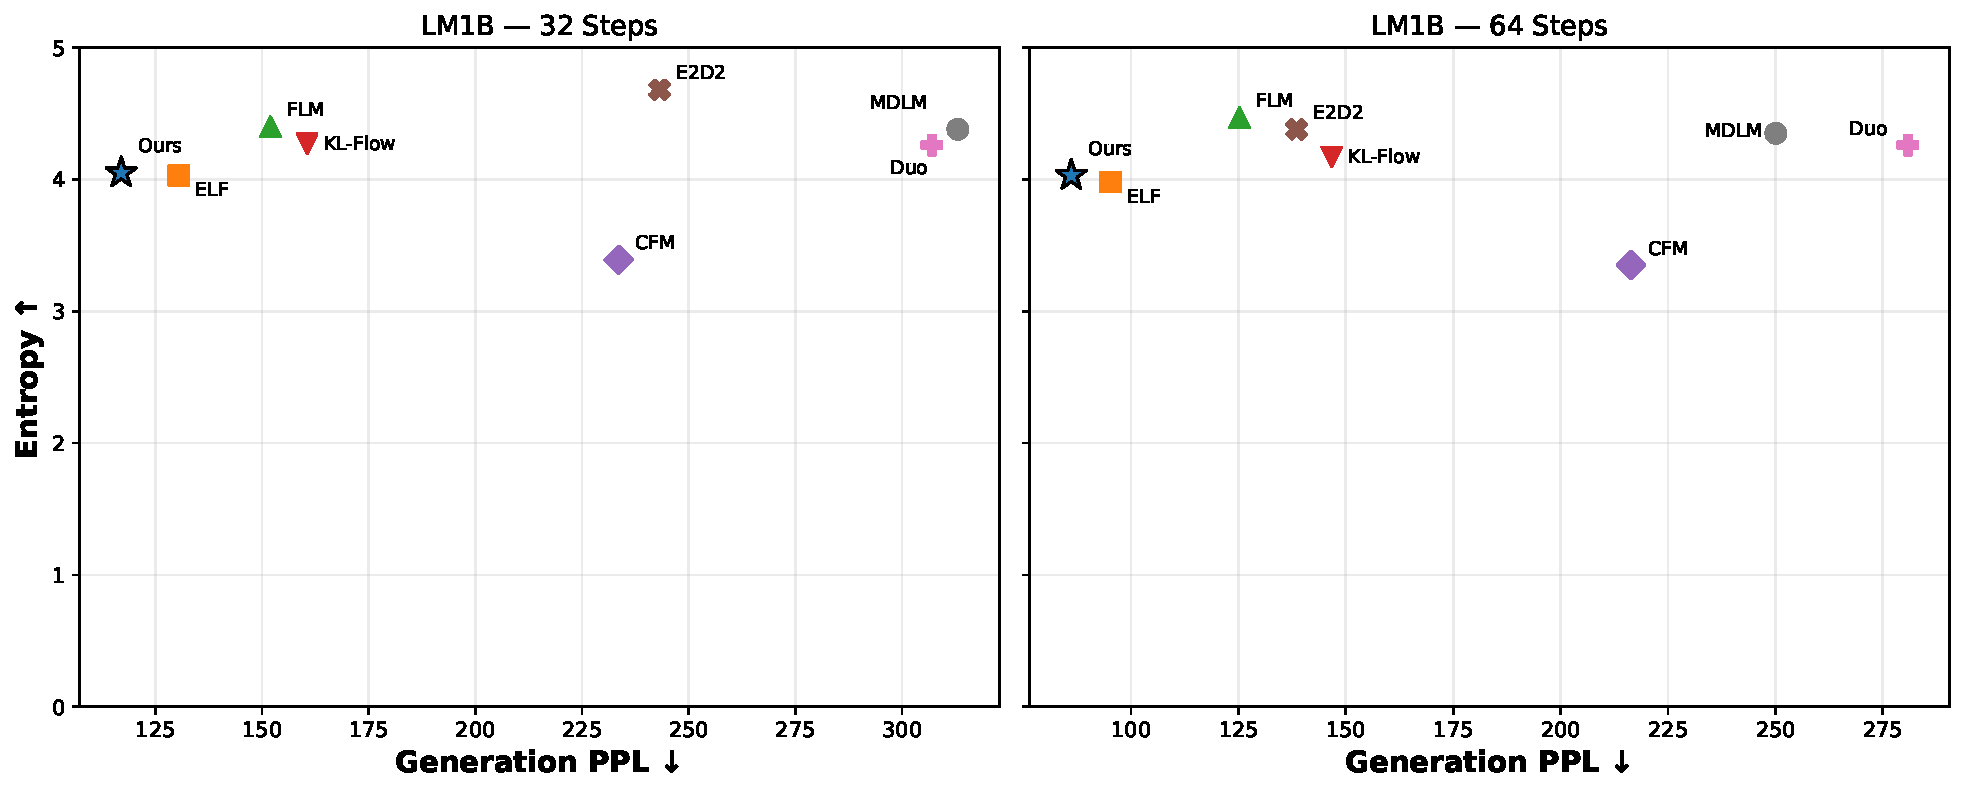
\includegraphics[width=\linewidth]{Figures/lm1b_32_64_scatter.pdf}
    \hspace{-5mm}
    \caption{Gen.~PPL--entropy trade-off on LM1B at 32 and 64 inference steps. Each point represents a competing method, with lower Gen.~PPL and higher entropy being preferred. Our method achieves the most favorable trade-off at both sampling budgets.}
    \label{fig:lm1b_32_64_scatter}
\end{figure}

\paragraph{OpenWebText.}
Table~\ref{tab:owt_results} reports the results (mean $\pm$ std) on OpenWebText under both 32- and 64-step sampling budgets. Our method consistently achieves the lowest Gen. PPL among all competing approaches, demonstrating improved generation fluency across different numbers of sampling steps. Compared with the strongest Flow Matching baseline, ELF~\citep{hu2026elf}, the improvement remains consistent at both sampling budgets. Meanwhile, the entropy of our samples remains comparable to ELF, with only a modest reduction in diversity. Overall, these results indicate that the proposed method improves generation quality while largely preserving sample diversity.

\begin{table}[t]
    \centering
    \begin{tabular}{l|cc|cc}
        \toprule
        & \multicolumn{2}{c|}{\textbf{32 Steps}}
        & \multicolumn{2}{c}{\textbf{64 Steps}} \\
        \cmidrule(lr){2-3}
        \cmidrule(lr){4-5}
        \textbf{Method}
        & \textbf{Gen. PPL $\downarrow$}
        & \textbf{Entropy $\uparrow$}
        & \textbf{Gen. PPL $\downarrow$}
        & \textbf{Entropy $\uparrow$} \\
        \midrule
        FLM~\cite{lee2026flowmaplanguagemodels}     & 244.68 \std{13.15}& 5.71 \std{0.03}  & 149.31 \std{8.63} & 5.68 \std{0.03} \\
        KL-Flow~\citep{sevriugov2026logitklflowmatchingnonautoregressive} & 241.60 \std{9.57} & 4.95 \std{0.04}  & 165.20 \std{8.23} & 4.86 \std{0.02} \\
        MDLM\citep{sahoo2024simple}    & 153.77 \std{8.90} & 5.69 \std{0.04}  & 104.52 \std{5.31} & 5.63 \std{0.03} \\
        CFM~\citep{roos2026categoricalflowmaps} & 167.10 \std{9.32} & 6.29 \std{004}  & 186.00 \std{9.74} & 6.41 \std{0.03} \\
        Duo~\citep{sahoo2025diffusionduality}      & 94.45 \std{5.46} & 5.57 \std{0.03}  & 85.27 \std{4.93}  & 5.56 \std{0.02} \\
        E2D2~\citep{arriola2025encoderdecoderdiffusionlanguagemodels}    & 36.24 \std{0.73}  & 2.57 \std{0.02}  & 28.01 \std{0.69}  & 2.27 \std{0.02}\\
        ELF~\citep{hu2026elf}     & 24.38 \std{1.05}  & 5.16 \std{0.03} & 19.31 \std{0.71}  & 5.08 \std{0.03} \\
        \midrule
        \textbf{Ours}
        & \textbf{18.84} \std{1.09} & 5.08 \std{0.03}
        & \textbf{14.97}\std{0.67} & 4.98 \std{0.03} \\
        \bottomrule
    \end{tabular}
    \caption{Results on OpenWebText with 32 and 64 sampling steps. Lower Gen. PPL indicates better fluency, while higher entropy indicates greater sample diversity. The results are conducted under 5 independent runs. Our method achieves the best perplexity (.PPL) while maintaining competitive diversity (Entropy).}
    \label{tab:owt_results}
\end{table}


\paragraph{LM1B.}
Table~\ref{tab:lm1b_results} reports the results (mean $\pm$ std) on LM1B under 32- and 64-step sampling budgets. Our method consistently achieves the lowest Gen. PPL across both settings, demonstrating improved generation quality over the competing approaches. At the same time, the entropy of the generated samples remains competitive across both sampling budgets, indicating that the improvement in perplexity does not come at the cost of a substantial reduction in diversity. These results further support the effectiveness of the proposed correlation-aware flow for unconditional language generation.

\begin{table}[t]
    \centering
    \begin{tabular}{l|cc|cc}
        \toprule
        & \multicolumn{2}{c|}{\textbf{32 Steps}}
        & \multicolumn{2}{c}{\textbf{64 Steps}} \\
        \cmidrule(lr){2-3}
        \cmidrule(lr){4-5}
        \textbf{Method}
        & \textbf{Gen. PPL $\downarrow$}
        & \textbf{Entropy $\uparrow$}
        & \textbf{Gen. PPL $\downarrow$}
        & \textbf{Entropy $\uparrow$} \\
        \midrule
        MDLM~\citep{sahoo2024simple}
        & 313.10 \std{12.71} & 4.38 \std{0.02}
        & 250.10 \std{10.17} & 4.35 \std{0.03} \\
        Duo~\citep{sahoo2025diffusionduality}
        & 306.99\std{12.45} & 4.26\std{0.03}
        & 280.83\std{11.37} & 4.26\std{0.03} \\
        E2D2~\citep{arriola2025encoderdecoderdiffusionlanguagemodels}
        & 243.21 \std{9.83} & 4.68\std{0.03}
        & 138.57\std{5.68} & 4.38\std{0.03} \\
        CFM~\citep{roos2026categoricalflowmaps}
        & 233.60\std{8.60} & 3.39\std{0.04}
        & 216.40\std{8.54} & 3.35\std{0.03} \\
        KL-Flow~\citep{sevriugov2026logitklflowmatchingnonautoregressive}
        & 160.60\std{6.47} & 4.27 \std{0.03}
        & 146.70\std{6.45} & 4.17 \std{0.02}\\

        FLM~\citep{lee2026flowmaplanguagemodels}
        & 152.01\std{6.12} & 4.40\std{0.04}
        & 125.24\std{6.09} & 4.47\std{0.03} \\
        
        ELF~\citep{hu2026elf}
        & 130.50\std{5.32} & 4.03\std{0.03}
        & 95.29\std{4.71} & 3.98\std{0.02} \\

        \midrule
        \textbf{Ours}
        & \textbf{117.03} \std{4.76} & 4.05 \std{0.04}
        & \textbf{86.09} \std{3.80} & 4.03 \std{0.03}\\
        \bottomrule
    \end{tabular}
    \caption{Results on LM1B with 32 and 64 sampling steps. Lower Gen. PPL indicates better fluency, while higher entropy indicates greater sample diversity. The results are conducted under 5 independent runs. Our method achieves the best perplexity (PPL) while maintaining competitive diversity.}
    \label{tab:lm1b_results}
\end{table}

\subsection{Ablation study}
\label{sec:ablation_study}

\begin{table}[t]
    \centering
    \begin{tabular}{l|cc|cc}
        \toprule
        & \multicolumn{2}{c|}{\textbf{32 Steps}}
        & \multicolumn{2}{c}{\textbf{64 Steps}} \\
        \cmidrule(lr){2-3}
        \cmidrule(lr){4-5}
        \textbf{Variant}
        & \textbf{Gen. PPL $\downarrow$}
        & \textbf{Entropy $\uparrow$}
        & \textbf{Gen. PPL $\downarrow$}
        & \textbf{Entropy $\uparrow$} \\
        \midrule
        \textbf{w/o Stage 2}     & 24.38 \std{1.05}  & 5.16 \std{0.03} & 19.31  \std{0.71}  & 5.08 \std{0.03} \\
        \textbf{w/o CorrNet}
        & 23.13 \std{1.04} & 5.02 \std{0.02}
        & 17.75 \std{0.65} & 4.92 \std{0.03} \\
        \textbf{w/o GP}
        & 20.44 \std{1.08}& 4.44 \std{0.04}
        & 17.72\std{0.68} & 4.19 \std{0.04}\\

        \midrule
        \textbf{Our}
        & \textbf{18.84} \std{1.09} & 5.08 \std{0.03}
        & \textbf{14.97}\std{0.67} & 4.98 \std{0.03} \\
        \bottomrule
    \end{tabular}
    \caption{Component-wise ablation on OpenWebText. 
    \textbf{w/o CorrNet} directly adapts the Flow Matching backbone to the GP path, while \textbf{w/o GP} trains the correlation network using the standard linear path. \textbf{w/o Stage 2} only train the standard Flow model $\theta$ in Stage 1.}
    \label{tab:ablation_component_owt}
\end{table}

\begin{table}[t]
    \centering
    \begin{tabular}{l|cc|cc}
        \toprule
        & \multicolumn{2}{c|}{\textbf{32 Steps}}
        & \multicolumn{2}{c}{\textbf{64 Steps}} \\
        \cmidrule(lr){2-3}
        \cmidrule(lr){4-5}
        \textbf{Variant}
        & \textbf{Gen. PPL $\downarrow$}
        & \textbf{Entropy $\uparrow$}
        & \textbf{Gen. PPL $\downarrow$}
        & \textbf{Entropy $\uparrow$} \\
        \midrule

        \textbf{w/o Stage 2}
        & 130.50 \std{5.32} & 4.03 \std{0.03}
        & 95.29 \std{4.71} & 3.98 \std{0.02} \\

        \textbf{w/o CorrNet}
        & 123.48 \std{5.21} & 3.93 \std{0.03}
        & 95.04 \std{3.84} & 3.90 \std{0.02} \\

        \textbf{w/o GP}
        & 136.44 \std{4.82} & 4.04 \std{0.03}
        & 102.81 \std{3.76} & 3.99 \std{0.03} \\

        \midrule
        \textbf{Our}
        & \textbf{117.03} \std{4.76} & 4.05 \std{0.04}
        & \textbf{86.09} \std{3.80} & 4.03 \std{0.03} \\

        \bottomrule
    \end{tabular}
    \caption{Component-wise ablation on LM1B.
    \textbf{w/o CorrNet} directly adapts the Flow Matching backbone to the GP path,
    while \textbf{w/o GP} trains the correlation network using the standard linear path.
    \textbf{w/o Stage 2} uses only the standard Flow Matching model trained in Stage~1.}
    \label{tab:ablation_component_lm1b}
\end{table}


\paragraph{Component-wise Contribution.}
Tables~\ref{tab:ablation_component_owt} and \ref{tab:ablation_component_lm1b} examine the individual contributions of the correlated GP path and the correlation network. Removing either component consistently degrades Gen.~PPL across both datasets and sampling budgets, while the full model achieves the best generation quality in all settings. Using the GP path without the correlation network already provides a meaningful improvement, showing the benefit of introducing a correlation-aware transport path. Conversely, using the correlation network without the GP path is not sufficient to recover the performance of the full model, indicating that the gain does not arise merely from adding extra model capacity. Notably, on OpenWebText, simply adding the correlation network and continuing training with the standard linear path leads to a clear drop in entropy, suggesting that the correlation network alone can harm sample diversity when it is not guided by the structured GP transport target. Together, these results show that the GP path and correlation network play complementary roles: the former provides a structured context-dependent transport target, while the latter provides an efficient mechanism for learning its corresponding velocity correction.

\paragraph{Sensitivity Analysis.}
We study the sensitivity of our method to the GP kernel, length scale, and context-window length in Tables~\ref{tab:kernel_sensitivity} and~\ref{tab:context_sensitivity}. Across different kernel types and length scales, the performance remains relatively stable, suggesting that the proposed method does not rely strongly on a particular GP hyperparameter configuration. Similarly, varying the context-window length leads to consistent performance and relatively stable entropy across both OpenWebText and LM1B. Overall, these results indicate that the method is robust to its main hyperparameter choices, while benefiting from a sufficiently informative local context.


\begin{table}[t]
    \centering
    \begin{tabular}{lc|c|ccc}
        \toprule
        & & \textbf{WMT14}
        & \multicolumn{3}{c}{\textbf{XSum}} \\
        \cmidrule(lr){3-3}
        \cmidrule(lr){4-6}
        \textbf{Kernel}
        & \textbf{Length scale $\ell$}
        & \textbf{BLEU $\uparrow$}
        & \textbf{ROUGE-1 $\uparrow$}
        & \textbf{ROUGE-2 $\uparrow$}
        & \textbf{ROUGE-L $\uparrow$} \\
        \midrule
        \textbf{RBF}
        & 0.25 & 25.99 \std{0.12}& 36.45 \std{0.09} & 12.98 \std{0.10} & 28.55 \std{0.11} \\
        & 0.50 & 25.98 \std{0.11}& 36.42\std{0.11} & 13.00 \std{0.012} & 28.55 \std{0.09} \\
        & 1.00 &  26.43 \std{0.13} & 36.41 \std{0.10} & 12.84 \std{0.12} & 28.51 \std{0.11} \\
        & 2.00 & 26.00 \std{0.11} & 36.40 \std{0.10} & 12.99 \std{0.11} & 28.52 \std{0.11} \\
        & 4.00 & 26.07 \std{0.13}& 36.39 \std{0.11} & 12.98 \std{0.12} & 28.53 \std{0.12} \\
        \midrule
        \textbf{Exponential}
        & 0.25 & 26.06 \std{0.12} & 36.56 \std{0.10} & 13.04 \std{0.11} & 28.58 \std{0.09} \\
        & 0.50 & 26.01\std{0.11} & 36.45 \std{0.11} & 13.02 \std{0.09} & 28.49 \std{0.10} \\
        & 1.00 & 26.12\std{0.08} & 36.41\std{0.10} & 12.95\std{0.09} & 28.06\std{0.09} \\
        & 2.00 & 25.97\std{0.11} & 36.11 \std{0.11} & 12.55\std{0.09} & 28.14 \std{0.10} \\
        & 4.00 & 26.47\std{0.13} & 35.96\std{0.12} & 12.48\std{0.12} & 28.08 \std{0.11} \\
        \bottomrule
    \end{tabular}
    \caption{Sensitivity to the GP kernel and length scale $\ell$ on
    WMT14 and XSum.  Higher BLEU and ROUGE scores are better.}
    \label{tab:kernel_sensitivity}
\end{table}

\begin{table}[t]
    \centering
    \small
    \begin{tabular}{c|cc|cc|cc|cc}
        \toprule
        & \multicolumn{4}{c|}{\textbf{OpenWebText}}
        & \multicolumn{4}{c}{\textbf{LM1B}} \\
        \cmidrule(lr){2-5}
        \cmidrule(lr){6-9}
        & \multicolumn{2}{c|}{\textbf{32 Steps}}
        & \multicolumn{2}{c|}{\textbf{64 Steps}}
        & \multicolumn{2}{c|}{\textbf{32 Steps}}
        & \multicolumn{2}{c}{\textbf{64 Steps}} \\
        \textbf{$n$}
        & \textbf{PPL $\downarrow$}
        & \textbf{Entropy $\uparrow$}
        & \textbf{PPL $\downarrow$}
        & \textbf{Entropy $\uparrow$}
        & \textbf{PPL $\downarrow$}
        & \textbf{Entropy $\uparrow$}
        & \textbf{PPL $\downarrow$}
        & \textbf{Entropy $\uparrow$} \\
        \midrule

        2
        & 21.21 & 5.074
        & 16.75 & 4.983
        & 125.14 & 4.041
        & 94.97 & 3.997 \\

      
        4
        & 23.56 & 5.124
        & 17.93 & 5.016
        & 124.15 & 4.003
        & 92.94 & 3.949 \\

        6
        & 23.92 & 5.161
        & 18.56 & 5.074
        & 128.11 & 4.061
        & 92.27 & 3.995 \\

        8
        & 18.84 & 5.154
        & 14.97 & 5.074
        & 117.03 & 4.049
        & 86.09 & 3.992 \\

        10
        & 20.69 & 5.135
        & 16.76 & 5.050
        & 119.67 & 4.094
        & 89.54 & 4.035 \\

        \bottomrule
    \end{tabular}
    \caption{Sensitivity to the context-window length $n$ on OpenWebText
    and LM1B under different sampling budgets. Lower Gen.~PPL indicates
    better generation quality, while higher entropy indicates greater
    sample diversity.}
    \label{tab:context_sensitivity}
\end{table}


\paragraph{Context Dependency Analysis.}
To examine whether the improvement arises from meaningful contextual
dependencies rather than the additional model capacity introduced by the
correlation network, we perform parameter-matched controls by replacing
its preceding-token context with zero or random inputs.
As shown in Table~\ref{tab:context_dependency}, using the true context
consistently yields substantially lower Gen.~PPL than both controls on
OpenWebText and LM1B across sampling budgets, while the entropy remains
comparable. These results indicate that the improvement is driven by the
contextual information captured by the proposed correlation mechanism,
rather than merely by introducing additional trainable parameters.


\begin{table}[t]
    \centering
    \begin{tabular}{ll|cc|cc}
        \toprule
        & & \multicolumn{2}{c|}{\textbf{32 Steps}}
        & \multicolumn{2}{c}{\textbf{64 Steps}} \\
        \cmidrule(lr){3-4}
        \cmidrule(lr){5-6}
        \textbf{Dataset}
        & \textbf{CorrNet Input}
        & \textbf{Gen. PPL $\downarrow$}
        & \textbf{Entropy $\uparrow$}
        & \textbf{Gen. PPL $\downarrow$}
        & \textbf{Entropy $\uparrow$} \\
        \midrule

        \multirow{3}{*}{OWT}
        & Zero context
        & 24.14 \std{1.08} & 5.14 \std{0.03}
        & 19.73 \std{0.57} & 4.99 \std{0.03} \\

        & Random context
        & 24.00  \std{1.12}& 5.10 \std{0.04}
        & 19.93 \std{0.62} & 4.92 \std{0.03} \\

        & \textbf{True context}
        & \textbf{18.84} \std{1.09} & 5.07 \std{0.03}
        & \textbf{14.97} \std{0.67} & 4.92 \std{0.03} \\

        \midrule

        \multirow{3}{*}{LM1B}
        & Zero context
        & 126.54 \std{4.83} & 4.05 \std{0.05}
        & 109.42 \std{3.97} & 4.01\std{0.04} \\

        & Random context
        & 136.46\std{4.62} & 4.06\std{0.04}
        & 105.51\std{4.21} & 4.01\std{0.03} \\

        & \textbf{True context}
        & \textbf{117.03}\std{4.76} & 4.05 \std{0.04}
        & \textbf{86.09}\std{3.80} & 4.03\std{0.03} \\

        \bottomrule
    \end{tabular}
    \caption{Context dependency analysis on OpenWebText and LM1B. 
    We replace the preceding-token context provided to the correlation
    network with either zero or random inputs while keeping the remaining
    model configuration unchanged.}
    \label{tab:context_dependency}
\end{table}


\paragraph{Scaling and Inference Analysis.} 
Figure~\ref{fig:scaling_analysis} examines the Gen.~PPL--Entropy trade-off
under different CorrNetwork and backbone capacities across inference
budgets. Increasing the CorrNetwork from the smallest to the intermediate
configuration improves the quality--diversity trade-off on both LM1B and
OpenWebText. However, further increasing its capacity by approximately
$2\times$ yields only marginal additional gains. A similar trend is
observed when scaling the base Flow Matching model: moving from the
smallest to the intermediate backbone improves the trade-off, whereas
further scaling provides limited benefit. Overall, these results suggest
that the proposed method benefits from additional capacity initially, but
quickly exhibits diminishing returns, indicating that strong performance
can be achieved without substantially increasing either the CorrNetwork
or the underlying backbone size.

\begin{figure}
    \centering
    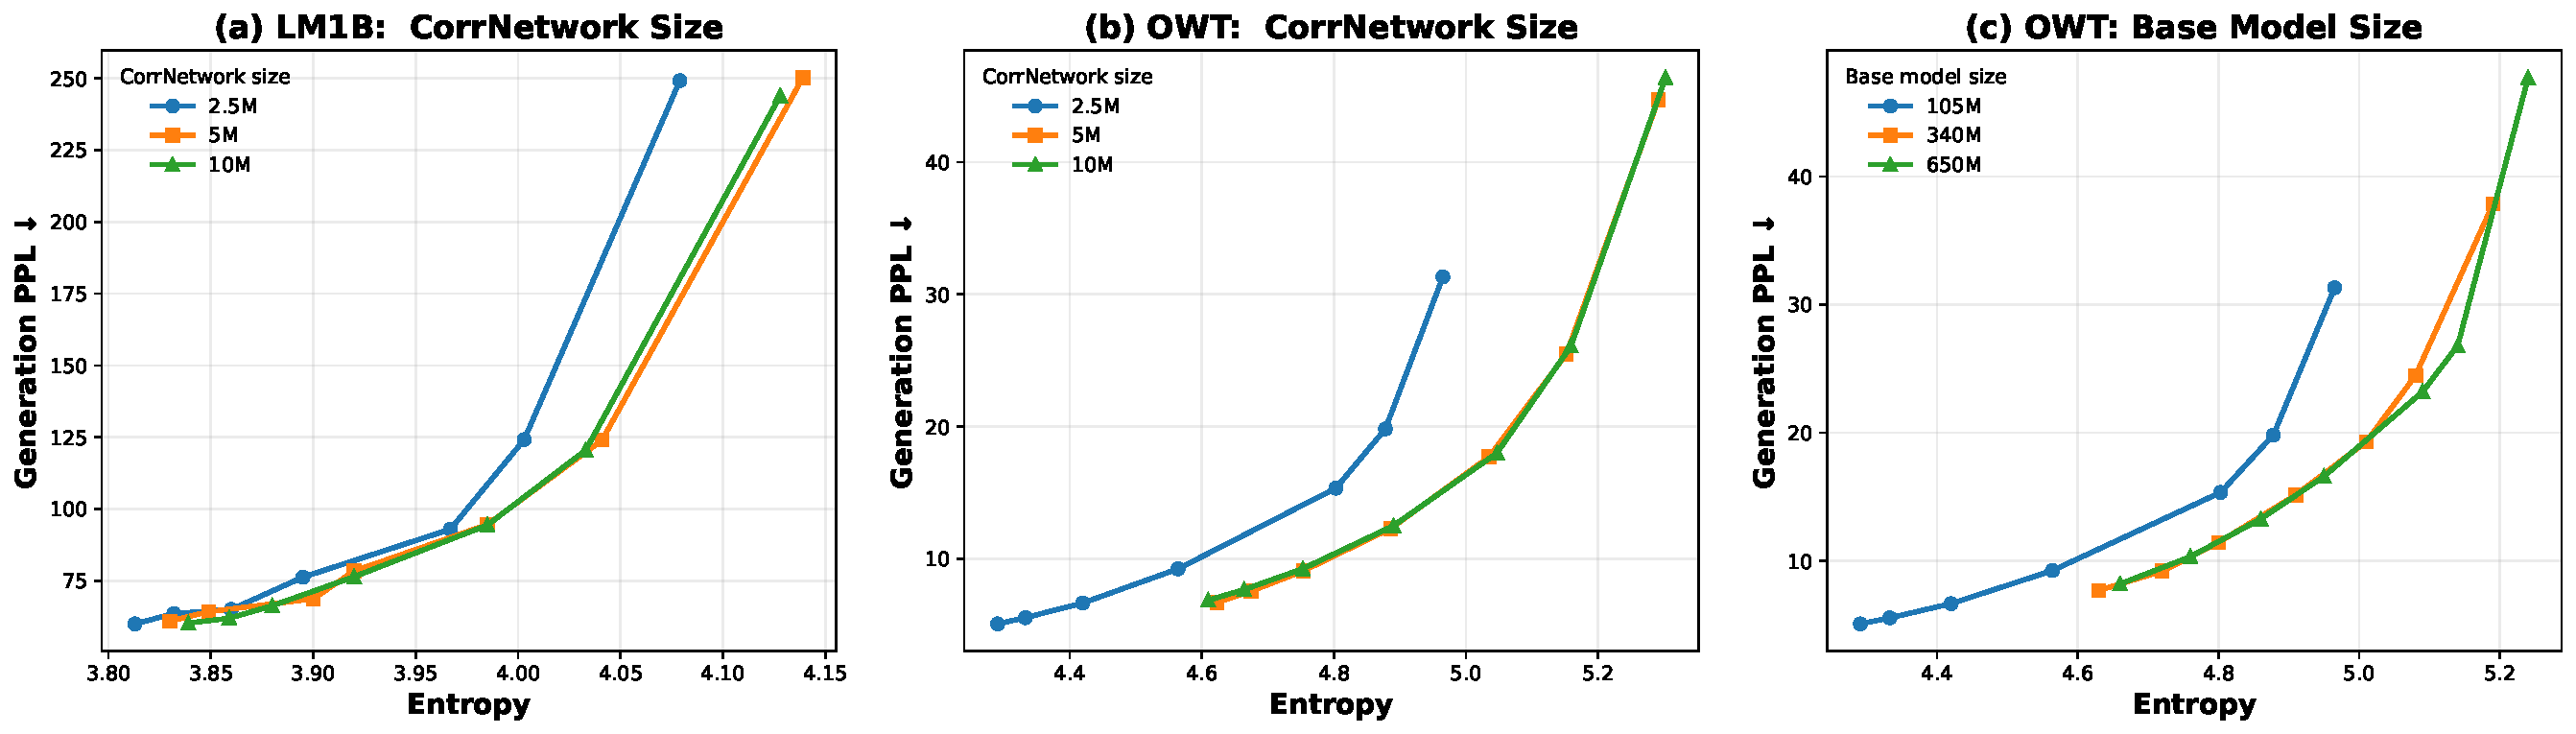
\includegraphics[width=\linewidth]{Figures/ppl_entropy_scaling_ablation.pdf}
    \caption{Gen.~PPL--Entropy trade-off under different model capacities and inference budgets. (a) LM1B with varying CorrNetwork sizes, (b) OpenWebText with varying CorrNetwork sizes, and (c) OpenWebText with varying base-model sizes. Lower Gen.~PPL and higher entropy are preferred. Increasing model capacity improves the trade-off initially, while further scaling yields diminishing returns.}
    \label{fig:scaling_analysis}
\end{figure}



\section{Discussion}
\label{sec:discussion}
This work highlights a broader perspective on flow-based language modeling:
the design of the transport process itself can play an important role in
representing linguistic dependencies. Existing approaches typically rely on
the neural velocity field to recover contextual interactions implicitly,
whereas our formulation introduces such structure directly into the transport
dynamics. The conditional-flow analysis provides a principled interpretation
of this design, showing that conditioning naturally induces an additional
context-dependent velocity component. Our GP-based correlated path and
lightweight correction network provide a practical way to realize this idea
while preserving the parallel nature of flow-based generation. More broadly, these results suggest that improving flow-based language models
may require not only stronger velocity networks or more sampling steps, but
also better structured probability paths that reflect the dependency structure
of language. This perspective opens a direction toward flow models whose
transport dynamics are explicitly designed around sequence structure rather
than treating token interactions solely as a function-approximation problem.

\section{Conclusions}
\label{sec:conclusion}
In this paper, we introduced Many-Body Language Flows (MLF), a correlation-aware framework that explicitly incorporates contextual dependencies into flow-based language generation. By combining a correlated transport path with a lightweight context-dependent velocity correction, MLF improves generation quality across both conditional and unconditional tasks while preserving the parallel nature of flow-based inference. These results suggest that explicitly structuring token interactions within the transport dynamics is a promising direction for improving flow-based language models.




\subsection*{Ethics statement}

(This section is \textbf{recommended} and does not count toward the page limit.)

If authors feel that their paper submission raises questions regarding the Code
of Ethics, they are encouraged to include a paragraph of Ethics Statement (at
the end of the main text before references) to address potential concerns where
appropriate. Topics include, but are not limited to, studies that involve human
subjects, practices to data set releases, potentially harmful insights,
methodologies and applications, potential conflicts of interest and sponsorship,
discrimination/bias/fairness concerns, privacy and security issues, legal
compliance, and research integrity issues (e.g., IRB, documentation, research
ethics). This statement should not be more than 1 page.

\subsection*{Reproducibility statement}

(This section is \textbf{recommended} and does not count toward the page limit.)

It is important that the work published in ICLR is reproducible. Authors are
strongly encouraged to include a paragraph-long Reproducibility Statement at the
end of the main text (before references) to discuss the efforts that have been
made to ensure reproducibility. This paragraph should not itself describe
details needed for reproducing the results, but rather reference the parts of
the main paper, appendix, and supplemental materials that will help with
reproducibility. For example, for novel models or algorithms, a link to an
anonymous downloadable source code can be submitted as supplementary materials;
for theoretical results, clear explanations of any assumptions and a complete
proof of the claims can be included in the appendix; for any datasets used in
the experiments, a complete description of the data processing steps can be
provided in the supplementary materials. Each of the above is an example of
things that can be referenced in the reproducibility statement.

% \subsubsection*{Author Contributions}
% If you'd like to, you may include  a section for author contributions as is done
% in many journals. This is optional and at the discretion of the authors.

% \subsubsection*{Acknowledgments}
% Use unnumbered third level headings for the acknowledgments. All
% acknowledgments, including those to funding agencies, go at the end of the paper.

\newpage
\bibliography{iclr2027_conference}
\bibliographystyle{iclr2027_conference}
\newpage
\appendix
\section{Appendix}
\subsection{Proof for Theorem~\ref{thm:conditional_flow}}
\label{sec:proof_ode_conditional}
\begin{proof}
 We define the density of the joint distribution as $\rho_{t}(\mathbf{x}, \mathbf{c})$, which satisfies
\begin{eqnarray}
    \partial_{t} \rho_t + \nabla_{\mathbf{x}} \cdot (\rho_t \vartheta_{\mathbf{x}}) + \nabla_{\mathbf{c}} \cdot (\rho_t \vartheta_{\mathbf{c}}) = 0 \label{eq:continuity_1}
\end{eqnarray}
Suppose the context $\mathbf{c}$ is observed, and $\mathbf{x}$ is to be generated. We define the marginal distribution over $\mathbf{c}$ as
\begin{eqnarray}
    \mathbf{m}_t (\mathbf{c}) = \int_{\mathbf{x}} \rho_t(\mathbf{x},  \mathbf{c}) d \mathbf{x}
\end{eqnarray}
Thus, we can compute the conditional distribution $\mathbf{q}_t (\mathbf{x} \mid \mathbf{c})$ as 
\begin{eqnarray}
    \mathbf{q}_t (\mathbf{x} \mid \mathbf{c}) = \frac{\rho_t(\mathbf{x}, \mathbf{c})}{\mathbf{m}_t (\mathbf{c})}
\end{eqnarray}
Taking the integral over $\mathbf{x}$ of ~\eqref{eq:continuity_1}, we have 
\begin{eqnarray}
    \partial_t \mathbf{m}_t + \int_{\mathbf{x}} \nabla_{\mathbf{x}} \cdot (\rho_t \vartheta_{\mathbf{x}}) d\mathbf{x} +  \nabla_{\mathbf{c}} \cdot \Big(\int_{\mathbf{x}}\rho_t \vartheta_{\mathbf{c}}  d\mathbf{x} \Big) =0 \label{eq:intergal_x}
\end{eqnarray}
Under vanishing-flux boundary conditions, the second term $\int_{\mathbf{x}} \nabla_{\mathbf{x}} \cdot (\rho_t \vartheta_{\mathbf{x}}) d\mathbf{x} = 0$. We then express the third term as 
\begin{eqnarray}
    \nabla_{\mathbf{c}} \cdot \Big(\int_{\mathbf{x}}\rho_t(\mathbf{x}, \mathbf{c}) \vartheta_{\mathbf{c}} (\mathbf{x}, \mathbf{c}, t)  d\mathbf{x} \Big) &= &\nabla_{\mathbf{c}} \cdot \Big(\mathbf{m}_t (\mathbf{c})\int_{\mathbf{x}}  \mathbf{q}_t (\mathbf{x} \mid \mathbf{c}) \vartheta_{\mathbf{c}} (\mathbf{x}, \mathbf{c}, t) d\mathbf{x} \Big) \\ \nonumber
    &= &\nabla_{\mathbf{c}} \cdot \Big(\mathbf{m}_t (\mathbf{c})) \mathbb{E}_{\mathbf{x}}  \big[ \vartheta_{\mathbf{c}} (\mathbf{x}, \mathbf{c},t )\mid \mathbf{c}\big]  \Big) \\ \nonumber
    &= & \nabla_{\mathbf{c}} \cdot \Big( \mathbf{m}_t (\mathbf{c}) \bar{\vartheta}_{\mathbf{c}} (\mathbf{c},t)\Big)
\end{eqnarray}
Thus, we can rewrite the~\eqref{eq:intergal_x} as 
\begin{eqnarray}
    \partial_t \mathbf{m}_t + \nabla_{\mathbf{c}} \cdot \Big( \mathbf{m}_t (\mathbf{c}) \bar{\vartheta}_{\mathbf{c}} (\mathbf{c},t) \Big) = 0 \label{eq:partial_m_t}
\end{eqnarray}
Substitution $\rho_t (\mathbf{x}, \mathbf{c}) = \mathbf{m}_t (\mathbf{c}) \mathbf{q}_t(\mathbf{x} \mid \mathbf{c}) $ into~\eqref{eq:continuity_1}, we get
\begin{eqnarray}
    \partial_t  \mathbf{m}_t \mathbf{q}_t +  \nabla_{\mathbf{x}} \cdot ( \mathbf{m}_t  \mathbf{q}_t\vartheta_{\mathbf{x}}) + \nabla_{\mathbf{c}} \cdot(\mathbf{m}_t\mathbf{q}_t  \vartheta_{\mathbf{c}}) &= &0  \\ \nonumber
    \mathbf{m}_t\partial_t \mathbf{q}_t  +  (\partial_t  \mathbf{m}_t)\mathbf{q}_t +  \mathbf{m}_t\nabla_{\mathbf{x}} \cdot (\mathbf{q}_t  \vartheta_{\mathbf{x}}) + \nabla_{\mathbf{c}} \cdot(\mathbf{m}_t\mathbf{q}_t  \vartheta_{\mathbf{c}})&= &0 \\ \nonumber
    \partial_t \mathbf{q}_t + \nabla_{\mathbf{x}} \cdot (\mathbf{q}_t \vartheta_{\mathbf{x}}) + \mathbf{m}^{-1}_t \big[ (\partial_t  \mathbf{m}_t)\mathbf{q}_t + \nabla_{\mathbf{c}} \cdot (\mathbf{m}_t\mathbf{q}_t  \vartheta_{\mathbf{c}})\big] &= &0 \\ \nonumber
\end{eqnarray}

Denoting $\mathbf{S}_t(\mathbf{x}, \mathbf{c}) = \mathbf{m}^{-1}_t(\mathbf{c}) \big[ (\partial_t  \mathbf{m}_t (\mathbf{c}))\mathbf{q}_t(\mathbf{x} \mid \mathbf{c}) + \nabla_{\mathbf{c}} (\mathbf{m}_t (\mathbf{c})\mathbf{q}_t (\mathbf{x} \mid \mathbf{c}) \vartheta_{\mathbf{c}}(\mathbf{x}, \mathbf{c}, t))\big]$, we have 
\begin{eqnarray}
    \partial_t \mathbf{q}_t + \nabla_{\mathbf{x}} \cdot (\mathbf{q}_t \vartheta_{\mathbf{x}})  + \mathbf{S}_t = 0 \label{eq:before_s}
\end{eqnarray}
Taking the integral over $\mathbf{x}$ of $\mathbf{S}_t(\mathbf{x}, \mathbf{c})$, we have 
\begin{eqnarray}
   \int_{\mathbf{x}} \mathbf{S}_t(\mathbf{x}, \mathbf{c}) d \mathbf{x} &=& \int_{\mathbf{x}} \mathbf{m}^{-1}_t \big[ (\partial_t  \mathbf{m}_t)\mathbf{q}_t + \nabla_{\mathbf{c}} \cdot(\mathbf{m}_t\mathbf{q}_t  \vartheta_{\mathbf{c}})] d\mathbf{x} \\ \nonumber
   &=& \mathbf{m}^{-1}_t  \Big[ (\partial_t  \mathbf{m}_t)\int_{\mathbf{x}}\mathbf{q}_t d\mathbf{x} + \nabla_{\mathbf{c}} \cdot \Big(\mathbf{m}_t \int_{\mathbf{x}} \mathbf{q}_t \vartheta_{\mathbf{c}} d\mathbf{x} \Big) \Big] \\
   &=& \mathbf{m}^{-1}_t  \Big[ (\partial_t  \mathbf{m}_t) + \nabla_{\mathbf{c}} \cdot \big(\mathbf{m}_t \bar{\vartheta}_{\mathbf{c}} \big) \Big]
\end{eqnarray}
Substitution~\eqref{eq:partial_m_t} into $(\partial_t  \mathbf{m}_t)$, we get
\begin{eqnarray}
  \int_{\mathbf{x}} \mathbf{S}_t (\mathbf{x}, \mathbf{c}) d \mathbf{x} &=& 0
\end{eqnarray}
It satisfies the compatibility condition for a no-flux divergence equation.
Assume that \(\mathbf{q}_t(\mathbf{x}\mid\mathbf{c})>0\) on the interior of the domain and that \(\mathbf{q}_t\) and \(\mathbf{S}_t\) are sufficiently regular and decay appropriately; there exists some $\mathbf{r}_t(\mathbf{x}, \mathbf{c})$ such that  
\begin{eqnarray}
    \mathbf{S}_t (\mathbf{x}, \mathbf{c}) = \nabla_{\mathbf{x}} \cdot \big(\mathbf{q}_t (\mathbf{x} \mid \mathbf{c}) \mathbf{r}_t (\mathbf{x}, \mathbf{c})\big) = \nabla_{\mathbf{x}}\cdot\big(\mathbf{q}_t \mathbf{r}_t \big) 
\end{eqnarray}
Here, we have 
\begin{eqnarray}
    \mathbf{m_t}\nabla_{\mathbf{x}} \cdot (\mathbf{q}_t \mathbf{r}_t) = [(\partial_t \mathbf{m}_t) \mathbf{q}_t + \nabla_{\mathbf{c}} \cdot (\mathbf{m}_t\mathbf{q}_t \vartheta_{\mathbf{c}})] \label{eq:define_r}
\end{eqnarray}
We can rewrite the~\eqref{eq:before_s} as
\begin{eqnarray}
    \partial_{t} \mathbf{q}_t + \nabla_{\mathbf{x}} \cdot (\mathbf{q}_t \vartheta_{\mathbf{x}}) + \nabla_{\mathbf{x}} \cdot (\mathbf{q}_t  \mathbf{r}_t ) &=& 0 \\ \nonumber
    \partial_{t} \mathbf{q}_t + \nabla_{\mathbf{x}} \cdot \Big(\mathbf{q}_t (\vartheta_{\mathbf{x}} + \mathbf{r}_{t}) \Big) &=& 0
\end{eqnarray}
This is the continuity equation with the conditional distribution $\mathbf{q}_t (\mathbf{x} \mid \mathbf{c})$. Therefore, the conditional distribution $\mathbf{q}_t(\mathbf{x}\mid\mathbf{c})$ is transported by the corrected velocity field as
\begin{eqnarray}
    \vartheta'_{\mathbf{x}}(\mathbf{x},t \mid \mathbf{c}) = \vartheta_{\mathbf{x}}(\mathbf{x}, \mathbf{c}, t) + \mathbf{r}_t (\mathbf{x}, \mathbf{c})
\end{eqnarray}

The correction $\mathbf{r}_t$ is generally non-unique, since any additional field $\mathbf{w}_t$ satisfying
\begin{eqnarray}
    \nabla_{\mathbf{x}}\cdot\big(\mathbf{q}_t\mathbf{w}_t\big)=0 \nonumber
\end{eqnarray}
produces the same conditional density evolution.
\end{proof}

\subsection{Detailed Experiment setup and hyperparameters}
\label{sec:implementation_details}
The experiments are conducted with 5 independent runs on the NVIDIA H100. Our anonymized code repository can be found at

\end{document}
